%%%%%%%%%%%%%%%%%%%%%%%%%%%%%%%%%%%%%%%%%%%%%%%%%%%%%%%%%%%%%%%%%%%
%                                                                 %
%                            ROOT FILE                            %
%                                                                 %
%%%%%%%%%%%%%%%%%%%%%%%%%%%%%%%%%%%%%%%%%%%%%%%%%%%%%%%%%%%%%%%%%%%
%
%  Run LaTeX or pdfLaTeX on this file to produce your thesis.
%  To produce the abstract title page followed by the abstract,
%  see the file abstitle-phd.tex or abstitle-mas.tex.
%
%%%%%%%%%%%%%%%%%%%%%%%%%%%%%%%%%%%%%%%%%%%%%%%%%%%%%%%%%%%%%%%%%%%

\documentclass[chap]{thesis}

% Use the first command below if you want captions over 1 line indented. A side
% effect of this is to remove the use of bold for captions (thesis default).
% To restore bold, also include the second line below.
\usepackage[hang]{caption}      % to indent subsequent lines of captions
\renewcommand{\captionfont}{\bfseries} % bold caption (needed with caption
                                       % package to restore boldface.)
%\includeonly{rpichap1}  % use \includeonly to process only
                         % the file(s) listed inside the braces

%Dan: color is used for notes to self while writing
\usepackage{color}
%Dan: for figures !
\usepackage[draft]{graphicx}
%Dan: for math !
\usepackage{amsfonts}
%Dan: for algorithms !
%Dan: these two by default define the same symbols...
% \usepackage{algpseudocode}
\usepackage{algorithm2e}
%Dan: for Seegyoung's drawings....
\usepackage{tikz}
\usetikzlibrary{decorations.pathmorphing}
\usetikzlibrary{arrows}
\usetikzlibrary{shapes.geometric}

\begin{document}

%\include{rpititle-mas}   % titlepage material for Master's thesis or project
%%%%%%%%%%%%%%%%%%%%%%%%%%%%%%%%%%%%%%%%%%%%%%%%%%%%%%%%%%%%%%%%%%%
%                                                                 %
%                            TITLE PAGE                           %
%                            PhD Thesis                           %
%                                                                 %
%%%%%%%%%%%%%%%%%%%%%%%%%%%%%%%%%%%%%%%%%%%%%%%%%%%%%%%%%%%%%%%%%%%
%  This file produces the title page, copyright page (if requested)
%  and the Table of Contents, List of Figures and List of Tables.
%
%  To produce the abstract title page followed by the abstract,
%  see the template file, "abstitle-phd.tex"
%%%%%%%%%%%%%%%%%%%%%%%%%%%%%%%%%%%%%%%%%%%%%%%%%%%%%%%%%%%%%%%%%%%

% Supply information for use on title page:
%
\thesistitle{\bf Conformal Simplex Mesh Adaptation\\On Heterogeneous Supercomputers}
\author{Daniel Ibanez}
\degree{Doctor of Philosophy}
\department{Computer Science} % provide your area of study here; e.g.,
%  "Mechanical Engineering", "Nuclear Engineering", "Physics", etc.

\signaturelines{4}     %max number of signature lines is 7
\thadviser{Mark S. Shephard}
 %\cothadviser{Second Adviser} % If you have 2 thesis advisers
\memberone{Onkar Sahni}
\membertwo{Christopher D. Carothers}
\memberthree{Elliot Anshelevich}
%\memberfour{Marcus Aurelius} % must change signaturelines to 5 if using this 5 members
%\memberfive{Marcus Junius Brutus} % must change signaturelines to 6 if using this 6 members
%\membersix{Nikola Tesla} % must change signaturelines to 7 if using this 7 members

\submitdate{Month 2016\\(For Graduation December 2016)}
\copyrightyear{2016}   % if omitted, current year is used.

% Print titlepage and other prefatory material:
%
\titlepage
\copyrightpage         % optional
\tableofcontents
\listoftables          % required if there are tables
\listoffigures         % required if there are figures


   % titlepage material for PhD thesis
%%%%%%%%%%%%%%%%%%%%%%%%%%%%%%%%%%%%%%%%%%%%%%%%%%%%%%%%%%%%%%%%%%%
%                                                                 %
%                         ACKNOWLEDGEMENT                         %
%                                                                 %
%%%%%%%%%%%%%%%%%%%%%%%%%%%%%%%%%%%%%%%%%%%%%%%%%%%%%%%%%%%%%%%%%%%

\specialhead{ACKNOWLEDGMENT}

This thesis owes its existence just as much to the support
and collaboration of numerous individuals as it does to
the efforts of the author.
My family must be thanked first for providing so much support
that I was able to give this thesis my full attention.
I must thank Prof. Mark S. Shephard as my mentor
for his unwavering support (and creation) of my career.
My doctoral committee have provided me with many insights:
Prof. Sahni on software development and the needs of advanced
CFD simulations, Prof. Carothers on the ever-changing landscape
of supercomputer architectures, Prof. Anshelevich on graph
theory's elegant solutions to practical problems,
and Prof. Shephard on how topology and adaptivity
can greatly improve existing simulations.

I am honored to have worked alongside students including
Cameron Smith, Brian Granzow, Daniel Zaide, Aleksandr Ovcharenko,
and others whom I consider comrades in the difficult trade
of developing good scientific software.
Other past and present members of SCOREC including Fabien
Delalondre, Seegyoung Seol, Max Bloomfield, and Assad Oberai
have provided guidance in life as well as work.

I admire and thank those who pioneer the adoption of mesh adaptation
in their important simulation workflows including Kenneth Jansen,
Michel Rasquin, Glen Hansen, Chris Kees, and Mike Park.

This thesis is built upon the decades of work by SCOREC including
that of Xiangrong Li, Rao Garimella, and Mark Beall.
It also owes much to the research in mesh adaptivity by
Fr{\'e}d{\'e}ric Alauzet, Adrien Loseille, and Jean-Fran{\c{c}}ois Remacle,
and in message passing by Torsten Hoefler, Andrew Lumsdaine,
and others.
  % include for acknowledgements
%%%%%%%%%%%%%%%%%%%%%%%%%%%%%%%%%%%%%%%%%%%%%%%%%%%%%%%%%%%%%%%%%%% 
%                                                                 %
%                            ABSTRACT                             %
%                                                                 %
%%%%%%%%%%%%%%%%%%%%%%%%%%%%%%%%%%%%%%%%%%%%%%%%%%%%%%%%%%%%%%%%%%% 
 
\specialhead{ABSTRACT}
 
This is a sentence used to take up space and look like text.
This is a sentence used to take up space and look like text.
This is a sentence used to take up space and look like text.
 
This is a sentence used to take up space and look like text.
This is a sentence used to take up space and look like text.
This is a sentence used to take up space and look like text.
This is a sentence used to take up space and look like text.
This is a sentence used to take up space and look like text.
This is a sentence used to take up space and look like text.
 
This is a sentence used to take up space and look like text.
This is a sentence used to take up space and look like text.
This is a sentence used to take up space and look like text.
This is a sentence used to take up space and look like text.
This is a sentence used to take up space and look like text.
This is a sentence used to take up space and look like text.
 
This is a sentence used to take up space and look like text.
This is a sentence used to take up space and look like text.
This is a sentence used to take up space and look like text.
This is a sentence used to take up space and look like text.
This is a sentence used to take up space and look like text.
This is a sentence used to take up space and look like text.
 % abstract
%%%%%%%%%%%%%%%%%%%%%%%%%%%%%%%%%%%%%%%%%%%%%%%%%%%%%%%%%%%%%%%%%%%
%                                                                 %
%                            CHAPTER ONE                          %
%                                                                 %
%%%%%%%%%%%%%%%%%%%%%%%%%%%%%%%%%%%%%%%%%%%%%%%%%%%%%%%%%%%%%%%%%%%

\chapter{INTRODUCTION AND BACKGROUND}
\label{chap:intro}

\section{Introduction}

A wide variety of aerospace, mechanical, and nuclear engineering
problems require solving complex Partial Differential
Equations (PDEs) in time and space.
For efficiency and reliability, the solutions to these PDEs are
found using computers.

Computers are equipped with a limited amount of memory to
store information, and must use a mathematical representation
of a PDE solution that can be described using
a limited amount of information.
For many engineering problems of interest, the exact solution
as described by any known representation would require an
infinite amount of information, therefore approximate
solutions are sought.

A certain minimal amount of memory and processing power
are required to obtain the lowest accuracy approximate
solutions, and obtaining more accurate solutions requires
more memory and/or processing power.
For these reasons, computers with ever-increasing amounts
of memory and processing power are designed and built to
increase the accuracy of existing solutions and
to solve previously unsolvable engineering problems.
At any given point in history, the computers with the
most memory and processing power are called supercomputers.

Supercomputers are expensive to acquire and even more
expensive to operate in terms of electricity, cooling, and other
maintenance, so their efficiency economic efficiency
at producing accurate results is of critical importance.

In the realm of PDE solutions, a discretization is an
approximate mathematical representation of a solution,
and many spatial discretizations are based on a mesh,
which is more precisely defined in Section \ref{sec:def_mesh}.
Chapter \ref{chap:struct} presents the full design
and implementation of two new computer representations
of meshes, which are focused on minimizing the amount
of computer memory and processing required to use
an accurate mesh, and are also compatible with mesh adaptation.

Mesh adaptation is a way in which the spatial discretization
(mesh) can be altered over time to maximize the accuracy
of the solution obtainable with a certain amount
of computing power.
There are several open areas of research in mesh adaptation,
and Chapter \ref{chap:adapt} presents advancements
made in this work to design and implement
mesh adaptation that can run efficiently on present
and near-future supercomputers.

Present supercomputers make extensive use of distributed
memory parallelism by being constructed from tens of thousands of
smaller computers (nodes) connected by a fast network.
In an effort to reduce acquisition and maintenance costs
for a given amount of computing power,
present and future supercomputers will also make extensive use
of shared memory parallelism, by having each node be constructed
with hundreds to thousands of computing cores, all of which
are capable of working in parallel.
The combination of the two forms of parallelism is what
makes a supercomputer \emph{heterogeneous}.

Designing programs for these supercomputers is a critical
challenge, because such programs must be able to precisely coordinate
a complex hierarchy totalling millions of compute cores
in order to solve a given problem at minimal cost.
Chapter \ref{chap:parallel} presents contributions to
the design and implementation of parallel programs,
including both widely applicable tools and tools specifically
designed to enable efficient parallel mesh adaptation.

An additional challenge to the design of parallel programs
is the fact that supercomputers fall into different
architectural design categories which currently
have very different programming interfaces.
Thus, in order to design a program which is \emph{portably performant}
over all architectures, one must try to abstract away
their differences and, unfortunately, cater to the
lowest common denominator of functionality.
Throughout this thesis, we present two systems:
the first only operates on some architectures and provides
a wide array of adaptive functionality, while the second
is portably performant across the major architectures
and provides less adaptive functionality.

Finally, Chapter \ref{chap:apps} presents several
application programs which make use of the tools developed
here in order to solve a variety of engineering problems.

\section{Nomenclature}

{\bf Part of the nomenclature is attributed to SISC}

\begin{tabular}{l|l}
Topological Complex & A breakdown of a domain in Cartesian space into
topological entities \\
Mesh & A topological complex whose entities have simple shape \\
Entity & A topological entity of a mesh \\
Vertex & A 0-dimensional entity \\
Edge & A 1-dimensional entity \\
Face & A 2-dimensional entity \\
Region & A 3-dimensional entity \\
Element & An entity not bounding another entity \\
\end{tabular}

\section{Definitions}

{\bf All definitions before hardware are from SISC}

\subsection{Topological Complex}

A point set is a subset of the points in some Cartesian
space $\mathbb{R}^D$.

A {\it topological complex} $T$ is a set of point sets
containing points in $\mathbb{R}^D$.
Each point set $T^d_i$ in $T$ is an open subset of some
$d$-dimensional manifold embedded in $\mathbb{R}^D$,
where $0\leq d \leq D$.
We say that $d$ is the dimension of point set $T^d_i$.
We can denote all point sets of dimension $d$ in the
complex by $T^d$.

All point sets in $T$ are disjoint from one another,
and their union $\Omega = \bigcup T$ is a subset of some $D$-dimensional
manifold, i.e. a $D$-dimensional manifold with boundary.
We denote the boundary of this complex as $\Gamma = \partial\Omega$.
Each point set is an open subset of a $d$-manifold,
and the closed equivalent on said manifold,
denoted $\bar{T}^d_i = T^d_i \cup \partial T^d_i$,
is the open set plus its boundary.
Since the sets are disjoint, only their boundaries may intersect.
For all pairs of equal-dimension point sets, the intersection
of their boundaries must exist as the union of other,
lower-dimensional point sets in $T$:

\[\forall T^d_i,T^d_{j\neq i} \in T: \exists S \subseteq \{T^q_k \in T \big| q < d\}:
\bigcup S = \partial T^d_i \cap \partial T^d_j\]

Finally, to keep the surface properly divided, we require that
the intersection of any point set boundary with the overall
boundary also exist as a union of lower-dimensional point sets:

\[\forall T^d_i \in T: \exists S \subseteq \{T^q_k \in T \big| q < d\}:
\bigcup S = \partial T^d_i \cap \Gamma\]

Boundary-representation (BRep) CAD models are examples
of topological complexes, as are meshes.
Point sets of dimension 0 are called vertices, those
of dimension 1 are called edges, faces have dimension 2
and regions have dimension 3.
When discussing a topological complex, we
refer to point sets as \emph{entities}.

\subsection{Adjacency Relation}
\label{sec:def_adj}

Given a topological complex $T$, we can describe the relations between
point sets in terms of adjacency.
If a point set $b$ bounds a point set $a$,
$b \subseteq \partial a$, then we say there is a
downward adjacency $(a,b)$.
Note that downward adjacency is a transitive relation:

\[c \subseteq \partial b, b \subseteq \partial a \to c \subseteq \partial a\]

For every downward adjacency $(a,b)$, there exists an upward
adjacency $(b,a)$.
Together, upward and downward adjacencies defined this way
are called first-order adjacencies.

The first-order adjacency relations in a mesh define a graph,
which we call a topology graph.
The majority of our work is concerned with finding
efficient computer representations for topology graphs.

The topology subgraph between a pair of dimensions $T^p$, $T^q$
is a bipartite graph.
We have a notation for queries of this bipartite graph:
$T^p_i\{T^q\}$ is the set of entities (point sets) in $T^q$ adjacent to
$T^p_i$.
In general, one can query all entities adjacent
to a set of entities: $S\{T^q\} = \bigcup a \{T^q\}, a \in S$.
This makes it easier to define second-order adjacencies,
which are found by two transitive queries,
for example $T^a_i\{T^b\}\{T^c\}$.

Although these graphs have a natural direction for each
edge (from higher dimension to lower), we are interested
in being able to query both outgoing (downward) and
incoming (upward) relations, so the storage will be
bi-directional in many cases.

Another useful concept will be the {\it entity use},
which is essentially an edge of the topology graph.
If entity $b$ is in the boundary of entity $a$, then
$b$ is used by $a$, and that occurrence is an entity use.
The term shows up when data is stored once for every adjacency relation.

\subsection{Mesh}
\label{sec:def_mesh}

A {\it mesh} $M$ is herein defined as a special case of a topological
complex where the closure of each entity $\bar{M}^d_i$
is topologically a polytope of dimesion $d$.
Mesh entities which do not bound other entities
are called \emph{elements}.

Being polytopes topologically, mesh entities have no
holes or internal empty spaces,
so they do not need multiple loop or shell constructs to
describe their boundary the way a BRep CAD model would.

\subsection{Finite Element Mesh}
\label{sec:def_fem}

We further define a {\it finite element mesh} as a special case
of a mesh, with certain restrictions and requirements.
For our current purposes, a finite element mesh is composed
of entities whose closures are one of the following
polytope types:

\begin{enumerate}
\item point $(d = 0)$
\item line $(d = 1)$
\item triangle $(d = 2)$
\item quadrilateral $(d = 2)$
\item tetrahedron $(d = 3)$
\item hexahedron $(d = 3)$
\item (square-based) pyramid $(d = 3)$
\item triangular prism $(d = 3)$
\end{enumerate}

This list can be easily extended to include additional polytope
types of interest.

This work is focused on \emph{unstructured meshes}, meaning
their topology must be explicitly stored because it
is not originally defined by some simple pattern such as a grid.
Such unstructured meshes have an
advantage in representing complex geometry and in their
ability to easily vary resolution throughout the geometry.

In addition, the Finite Element Method uses fields which are each defined
as the weighted sum of finite number of basis functions,
where the weights are referred to as \emph{degrees of freedom} and are each
attached to one mesh entity.
This requires a data structure that can attach
degrees of freedom to mesh entities.

Finite element analysis procedures also require meshes where
the number of elements around some boundary entity (such as a vertex
or an edge) is limited to a reasonable upper bound,
otherwise shape quality and numerical conditioning will degrade.
Therefore, in such meshes, all upward adjacencies are bound
by a constant.
Any operation whose runtime is proportional to the
number of upward adjacencies can be treated as a constant-time operation.

{\bf consider including a more detailed proof of constant upward
adjacency degree, which I already have written somewhere}

Finally, if there are multiple polytope types per dimension,
such as having both triangles and quadrilaterals in 2D, then
we say the mesh is {\it mixed}.

\subsection{Mesh Construction and Modification}

There are two approaches to modifying the topology throughout
a simulation.
If an entirely new mesh is constructed, we say that the
method is {\it remeshing}.
If local changes are applied to the original mesh to transform
it into the new mesh, we say the method {\it adapts}.
Such local changes require adding and removing entities
from the mesh within local portions of the domain.
On the other hand, if the mesh is not changed during the
simulation, we say that the mesh is {\it static}.

\subsection{Adaptation}
\label{sec:def_adapt}

Adaptation refers to a process of modifying the mesh by applying
mesh entity-level operations on mesh cavities.
We can define a {\it mesh cavity} as the
union of several mesh entities, in which the
mesh modification changes the interior (open set) of
the mesh entities within the cavity, leaving its boundary unchanged.

Adaptation has a number of benefits compared to complete remeshing.
Remeshing has a runtime cost at least proportional to the number
of total elements, while the cost of adaptation is only proportional
to the number of mesh entities modified.
Moreover, the transfer of field values from the old mesh
to the new mesh is a complex procedure when remeshing,
requiring spatial search algorithms and
tends to apply remapping operators that are diffusive and/or
have to deal with conservation requirements at a global level.

Adaptation by local mesh modification supports local execution
of solution transfer: refinement splits
parent entities and is able to transfer solution exactly using
shape function interpolation, and other operations are confined
to a local cavity so that any searching is fast,
and diffusive effects and conservation adjustments are local.

Local mesh adaptation requires unique properties of the
mesh data structure that are otherwise unnecessary for
static meshes.
Adaptive procedures are composed of a series of
mesh entity additions and removals.
Therefore, at a minimum, we require that \emph{entity
addition and removal be constant-time operations}.

For several reasons, it is preferable to modify a cavity
by first constructing all new entities that fill the cavity,
which overlap with the old, and then destroying all old entities.
First, this allows both versions to be considered by a solution
transfer algorithm, which needs the mesh topology from both
to operate properly in the general case.
Second, we are able to evaluate quality and correctness metrics
of the new entities and, if those are unacceptable, cancel the
operation by destroying the new entities and leaving
the old entities in place.

As a consequence, the mesh structure must \emph{tolerate temporary
topological inconsistencies} introduced by adaptation.
For example, the first modification made is either the addition
of an entity which overlaps with existing entities
or the removal of an entity.
Adding an overlapping entity causes inconsistencies such as
a face which has three adjacent regions in the temporary mesh.
Removing an arbitrary entity can cause non-manifold configurations,
such as that of a vertex adjacent to only two elements, which
in turn only intersect at that vertex.

Certain modifications, such as edge collapsing, can only correctly
preserve the boundary of the mesh the mesh structure \emph{maintains
a direct mapping from mesh entities to geometric (CAD) model
entities}.
This mapping is referred to as classification \cite{schroeder1990combined}.
For example, sharp edges
can be preserved when it is known that a mesh entity is
on such a CAD model edge.
The inverse map of classification is called reverse
classification, and it defines the groups of mesh entities
to which boundary conditions are applied.

The implementations of edge collapsing which preserve
topological similarity have so far required knowledge
of the classification for all mesh entities,
hence requiring a complete topological representation \cite{seol2006efficient}
to safely coarsen a mesh.
Beyond that, it is convenient in any case to represent
edges explicitly, given that many adaptive algorithms
are based on edge lengths \cite{biswas1998tetrahedral}.

\subsection{Petascale and Heterogeneous Supercomputers}

{\bf Define things like processors, ``node", accelerator, etc.}

\subsubsection{Programming Environments}

{\bf Define MPI, threads, CUDA terminology.}

This reference describes the CUDA environment: \cite{nickolls2008scalable}.

\section{Goals}
\label{sec:intro_goals}

{\bf These goals are from the SISC paper in review, will
need to be attributed}

An unstructured mesh simulation code relies heavily on
multiple core capabilities to deal with the mesh,
and the range of features available at this level constrain
the capabilities of the simulation as a whole.
As such, the long-term goal towards which this thesis
contributes is the development of a mesh handling system
with the following capabilities:

\begin{enumerate}
\item The flexibility to adapt to evolving meshes
\item The ability to represent any of the conforming meshes typically
used by Finite Element (FE) and Finite Volume (FV) methods
\item Low memory use
\item High locality of storage
\item Highly scalable implementation for distributed memory computers
\item The ability to parallelize work inside heterogeneous
supercomputer nodes
\end{enumerate}

The first goal is the most consequential; supporting adaptivity
is the reason for much of the complexity in the structure
and its difference compared to many non-adaptive mesh structures
(see Section \ref{sec:def_adapt} for further discussion).
In particular, we present a derivation for a family of structures
with the following properties:

\section{Overview of Software}

\subsection{PUMI}

The Parallel Unstructured Mesh Infrastructure (PUMI) is a software package
containing several libraries which together provide all the tooling
necessary to store, query, and adapt partitioned meshes with
simulation fields attached.
PUMI's design is based on locally serial software threads which
cooperate with one another using message passing, assuming
there is no sharing of memory.
Each software thread is required to have access to all computer
functions including memory allocation, message passing, file I/O, and the ability
to call any available third party library.
Because of these assumptions, PUMI's code could not execute
on more restricted architectures such as GPUs without very
substantial re-design and re-implementation.

\subsubsection{PCU}

PCU is a C library which implements the key parallel communication
systems required to construct more complex parallel programs
which remain scalable.
Its algorithms and implementation will be covered in detail
in Section \ref{sec:pcu}.
PCU uses MPI to transmit all its messages, making it portable
across many distributed memory supercomputers.

\subsubsection{APF}

APF is a C++ library whose original goal was to manage fields discretized
over a mesh.
In order to achieve that goal without being tied to a particular mesh
implementation, APF included an abstract interface for interacting
with any mesh implementation.
Because algorithms based on this interface are immediately able to
operate on multiple different mesh implementations, APF now contains
many such algorithms dealing with topological and parallel operations.

\subsubsection{MDS}

MDS is a C library implementing the main mesh data structure for APF and
therefore PUMI.
It is array-based, supports adding and removing entities in constant time,
can represent multiple element types at once, and is augmented with
parallel connectivity information for partitioned meshes.
This structure will be described in detail in Section \ref{sec:sisc}.

\subsubsection{MeshAdapt}

MeshAdapt is a C++ library that leverages PCU, APF, MDS, and other
libraries in PUMI to implement scalable parallel mesh adaptation.
MeshAdapt developments which are part of this thesis will be covered
in detail in Sections \ref{sec:ma_methods} as well as Section
\ref{sec:cavity_operator}.

\subsection{Omega\_h}

Omega\_h is a single C++ library which was designed from the beginning
with the restrictions and potential of GPU programming in mind.
It aims to provide as much of the core functionality of PUMI as
is feasible in a portably performant way, which currently
amounts to adapting triangle and tetrahedral meshes to anisotropic
metrics.
Omega\_h represents the first such portably performant code capable
of mesh adaptation, and is a major contribution of this thesis.
Its fundamental approach to on-node parallelism is
presented in Section \ref{sec:parallel_for}, and techniques
used to maintain deterministic execution are presented
in Section \ref{sec:determinism}.
Its data structure will be described in Section \ref{sec:omega_h-struct}.
Its implementation of mesh adaption will be discussed mainly
in Section \ref{sec:omega_h-adapt}, with key parallel aspects
covered throughout Chapter \ref{chap:parallel}.

\section{Related Works}

{\bf TODO: brief mention of each related work.}

%%% Local Variables:
%%% mode: latex
%%% TeX-master: t
%%% End:

%%%%%%%%%%%%%%%%%%%%%%%%%%%%%%%%%%%%%%%%%%%%%%%%%%%%%%%%%%%%%%%%%%%
%                                                                 %
%                            CHAPTER TWO                          %
%                                                                 %
%%%%%%%%%%%%%%%%%%%%%%%%%%%%%%%%%%%%%%%%%%%%%%%%%%%%%%%%%%%%%%%%%%%

\chapter{ARRAY-BASED MESH REPRESENTATIONS}
\label{chap:struct}

\section{Rationale}

Various requirements for storing of entities, adjacencies,
ability to modify.
Indicate how each requirement affects complexity.

\section{Related Work}

Specifics of mesh representations in the literature.
This can probably come from the SISC paper, plus
some more SCOREC references.

\section{Two Paradigms, Two Structures}

A lead-in describing the two structures and their difference
in abilities.

The end of this section can discuss possibilities of convergence.

\section{PUMI/APF Data Structure}

SISC paper on PUMI/APF structure goes here.

\section{Omega\_h Data Structure}

\subsection{Adjacency Cache}

\subsection{Alignment Codes}

\section{Data Structure Performance}

Query times, modification times, etc. for both structures.

%%% Local Variables:
%%% mode: latex
%%% TeX-master: t
%%% End:

%%%%%%%%%%%%%%%%%%%%%%%%%%%%%%%%%%%%%%%%%%%%%%%%%%%%%%%%%%%%%%%%%%%
%                                                                 %
%                            CHAPTER THREE                        %
%                                                                 %
%%%%%%%%%%%%%%%%%%%%%%%%%%%%%%%%%%%%%%%%%%%%%%%%%%%%%%%%%%%%%%%%%%%

\chapter{CAVITY-BASED CONFORMAL MESH ADAPTATION}
\label{chap:adapt}

\section{In Context}

The mesh adaptation methods in this work are
conformal, general, and cavity-based.

\subsection {Conformal and General}

They are conformal in the sense that the boundaries of all
elements (Section \ref{sec:def_complex}) are composed
of the set of entities expected by that element's
topological template (Section \ref{sec:topo_template}).
In other words, we avoid the ``hanging node" scenarios
introduced by non-conformal mesh modification techniques.
Typically, non-conformal mesh modification also restricts
itself to subdividing input elements into more elements,
or undoing such subdivisions which were done before.
Figure \ref{fig:hex_amr} illustrates such a method,
and clearly shows the hanging nodes introduced.

\begin{figure}
\begin{center}
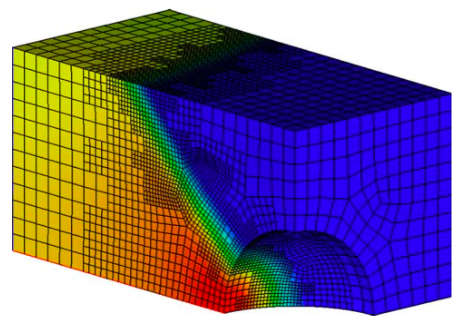
\includegraphics[width=0.6\textwidth]{hex_amr.png}
\caption{Non-conforming parent-child adaptive mesh refinement
\cite{kirk2006libmesh}}
\label{fig:hex_amr}
\end{center}
\end{figure}

Non-conforming meshes require additional support from
the PDE-solving code to deal with hanging nodes, and typically
no more than one level of refinement is allowed between adjacent
elements.
The more important limitation is due to non-conforming methods
typically being parent-child methods, which fundamentally limits
them to the topology (and geometry) of the coarse input mesh.
If this input mesh is more fine than necessary in some areas,
it cannot be coarsened.
If moving objects or object deformation cause input elements
to become highly compressed or even inverted, parent-child
refinement can never correct or prevent this.
New node placement when refining along a curved boundaries poses
a similar issue to that of physical deformation.
For these reasons we take a general approach, employing
coarsening, swapping, and possibly other operations which are
able to coarsen beyond the input mesh and correct low-quality
elements in the input mesh.

\subsection{Cavity-Based}

We restrict ourselves to local cavity operations as well,
meaning that the transformation from input to output meshes
can be expressed as a series of cavity modifications, each
of which can in turn be expressed as the removal of
a small number of mesh entities followed by the addition
of a small number of mesh entities.

In general, a cavity can be defined as a manifold sub-domain
of the mesh defined by a set of elements from the original
input mesh.
A cavity undergoes a modification, which changes the discretization
(set of mesh entities) of its interior but leaves its ``boundary" unchanged.
In order to allow changing the discretization of the overall
mesh boundary (i.e. the geometric model boundary)
we use a relaxed definition of a cavity boundary
(shown in Figure \ref{fig:cavity_boundary}) which only includes
entities that are also adjacent to elements outside the cavity.
This is the minimum requirement for the method to be conformal:
it must preserve the topology of this relaxed boundary.
For efficient parallel execution, we also require that attributes
of those boundary entities remain unchanged (this includes
geometric classification, hence Figure \ref{fig:surf_collapse}).
This allows two cavities to be modified simultaneously by two
threads or processes, so long as the cavities do not overlap
(i.e. they do not share elements).
They may be adjacent (share a subset of their boundaries) and
need not coordinate because nothing about the shared boundary
will be changed by either one.

\begin{figure}
\begin{center}
\includegraphics[width=0.6\textwidth]{cavity_boundary.png}
\caption{Relaxed definition of cavity boundary excludes geometric boundary}
\label{fig:cavity_boundary}
\end{center}
\end{figure}

Some benefits of using local cavity operations are:
\begin{enumerate}
\item It allows more straightforward and reliable parallelization of
mesh adaptation (see Section \ref{sec:cavity_sched}).
\item It allows much more careful control of the effects that mesh
adaptation has on the simulation fields attached to the mesh.
\end{enumerate}

On the other hand, the set of known cavity operations
have been found by the trial and error of researchers,
and there are many properties which they are not guaranteed to
achieve.
The most successful set of cavity operators are those
which operate on simplex meshes, due ultimately to the
fact that a simplex is the simplest polytope of a given dimension
and that, conversely, more complex polytopes provide fewer
valid configurations.
In our work, we separate cavity operators into several categories:
\begin{enumerate}
\item Refinement: create a strictly more detailed discretization
than the input. Guaranteed not to invert elements, but not to
preserve any element quality. Guaranteed to exactly preserve
the distribution of fields.
\item Coarsening: create a strictly less detailed discretization
than the input. No guarantees it can be done without reducing
or negating quality, so it must be checked.
By definition, cannot exactly preserve the distribution of the fields.
\item Shape correction: typically maintains similar level of detail,
modifies connectivity to improve minimum element quality.
There is no known method guaranteed to raise all elements to a quality
that is useful for simulation and adaptation, but heuristic
methods can achieve great results in practice \cite{klingner2008aggressive}.
\item Snapping: procedures intended to improve the discrete
mesh approximation of a continuous curved boundary.
\end{enumerate}

\section{Related Work}

There have been several iterations of the MeshAdapt
library developed at RPI.
One of the earliest publications by De Cougny and Shephard
\cite{de1999parallel} outlines the three basic steps and goes into some detail
on a use of independent sets for coarsening purposes
(an idea that we extend significantly in Section \ref{sec:indset}).
Later, substantial extensions were introduced by Li on anisotropy using the metric
tensor and the selection of operators for shape correction
\cite{li20053d,li2003mesh}.
Our implementations of tetrahedral edge swaps make use
of guidance on fast implementation by Olivier-Gooch \cite{freitag1997tetrahedral}.
Researchers at INRIA have provided useful mathematical foundations
for handling the anisotropic metric tensor field
\cite{frey2005,alauzet2006parallel,loseille2015parallel},
and work at the Catholic University of Louvain explored
the use of mesh adaptation to respond to moving objects
\cite{compere2010mesh}, a path we continue with our Omega\_h work.

\section{MeshAdapt Methods}
\label{sec:ma_methods}

\subsection{Template Refinement}
\label{sec:ma_refine}

The MeshAdapt library uses edge-based refinement templates for its refinement step.
The way these work is that all edges whose metric length exceeds some threshold
$l_{\text{up}} > 1$ are marked for refinement.
Then each element takes into account the subset of its edges which are marked
for refinement, and chooses one of many possible subdivision patterns
(refinement templates) based on this subset of edges.
Figure \ref{fig:tet_templates} illustrates these templates in the case of tetrahedra.
In fact, the center template shown for three marked edges has two variants which
are symmetric by reflection but not by rotation.
In total, this means there are 12 rotationally unique tetrahedron refinement templates.

\begin{figure}
\begin{center}
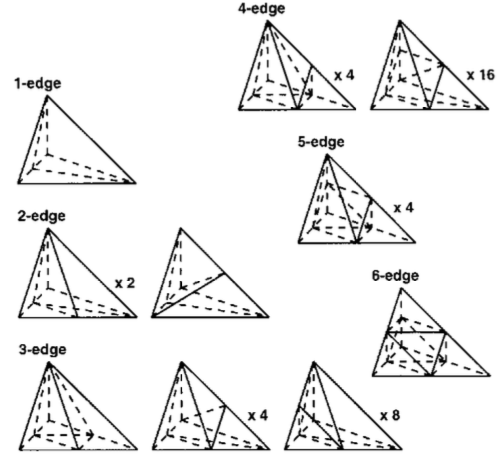
\includegraphics[width=0.6\textwidth]{tet_templates.png}
\caption{Tetrahedral refinement templates}
\label{fig:tet_templates}
\end{center}
\end{figure}

One benefit of the use of refinement templates is that adjacent elements can be refined
simultaneously, so all edges, faces, and regions of the mesh can be modified in
a nearly embarrassingly parallel fashion once the set of marked edges is identified.
Another benefit is that the gradation of the mesh is more explicitly controlled
compared to methods which split edges independently.
However, refinement templates have some drawbacks as well:
\begin{enumerate}
\item In some cases, a subset of the template is a polyhedron that cannot be
subdivided into tetrahedra without introducing an extra vertex within the
parent tetrahedron.
In particular, Sch{\"o}nhardt's polyhedron can appear (see Figure
\ref{fig:schonhardt}).
This reduces the predictability of refinement and makes it more difficult
to transfer solution.
\item Other cases introduce a geometric decision, such as the case
when all edges of a tetrahedron are refined, or even when two edges
of a triangle are refined. This also reduces predictability.
\item It takes substantial code to implement all rotationally unique
combinations for all the relevant element polytopes.
This increases the likelihood of errors and decreases the productivity
of modifying any aspect of refinement.
\item Due to the simultaneous nature of the operation and the difficulty
of predicting the outcome, it is prohibitively difficult to reject
a local portion of the refinement based on criteria such as new elements
having too low quality.
\end{enumerate}

\begin{figure}
\begin{center}
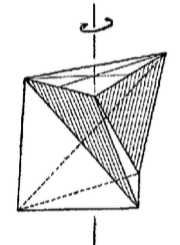
\includegraphics[width=0.2\textwidth]{schonhardt.png}
\caption{Sch{\"o}nhardt's irreducible polyhedron
\cite{Schonhardt1928}}
\label{fig:schonhardt}
\end{center}
\end{figure}

\subsection{Coarsening}
\label{sec:ma_coarsen}

Like other adaptation libraries, MeshAdapt implements
coarsening via edge collapses.
Figure \ref{fig:collapse} shows a typical edge collapse
in a tetrahedral mesh for reference.
One vertex in the mesh is ``moved" onto another vertex which is adjacent
via a mesh edge, collapsing this edge and all its adjacent
faces and regions.
For programming purposes, when dealing with sets of entities we
can call those being removed the ``collapsing" set and those being
conceptually elongated to fill the cavity as the set to ``keep".
In practice all old entities are removed and the set of entities to keep
is rebuilt with modified connectivity (where they were adjacent to the
collapsed vertex, now they are adjacent to the kept vertex).

\begin{figure}
\begin{center}
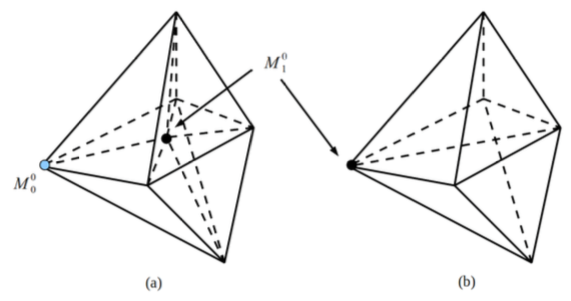
\includegraphics[width=0.6\textwidth]{collapse.png}
\caption{Edge collapse in tetrahedral mesh
\cite{lu2011developments}}
\label{fig:collapse}
\end{center}
\end{figure}

Edge collapsing is an operation which, if not properly controlled,
can invalidate the mesh topologically or undo its topological similarity
to a CAD model \cite{schroeder1990combined}.
MeshAdapt uses a set of checks which is somewhat expensive to compute
but is topologically robust:

\begin{enumerate}
\item The vertex being collapsed must have the same classification as
the edge being collapsed. This preserves similarity to the CAD model by
preventing collapses from the boundary into the interior.
\item If there exists a ring of three edges including the collapsing edge
(Figure \ref{fig:edge_ring}),
then those three edges must bound a single triangle in the mesh.
This prevents collapsing an empty hole in the mesh to zero volume as in
Figure \ref{fig:circle_hole}.
While some \cite{beall1997general} consider Figure \ref{fig:circle_hole}
a valid operation, current mesh data structures assume an entity is uniquely
defined by its set of bounding entities, which precludes the two overlapping
mesh edges that Figure \ref{fig:circle_hole} produces.
In addition, the non-collapsing edge adjacent to the collapsing vertex must have the same
classification as the triangle.
This prevents collapsing a cavity on a curved boundary down to zero volume
(see Figure \ref{fig:surf_collapse}), which would require re-classifying
entities on the cavity boundary (which breaks parallelism guarantees), and
creates no elements in the new cavity (which is problematic for solution transfer).
\item Analogous to the edge ring check, in 3D we check for two triangles which
share a non-collapsing edge and whose remaining two vertices are the endpoints
of the collapsing edge (a ``face ring").
The two triangles and the collapsing edge must bound a single tetrahedron,
and the triangle adjacent to the collapsing vertex must have the same classification
as this tetrahedron.
\item All the resulting tetrahedra must have positive volume.
In the 2D planar case, triangle normals should all be positive in the Z axis.
A relaxed version of this can be used to adapt triangulations of 2D surfaces
embedded in 3D, by requiring that the normals of new triangles be sufficiently
close to the normals of old triangles.
For straight-sided simplices in an equal-dimensional space (i.e. triangles in 2D),
this check on its own can prevent some topological invalidities, except
those in Figure \ref{fig:circle_hole} and Figure \ref{fig:surf_collapse}.
\end{enumerate}

The edge and face ring conditions are more complete versions of those described
by Garimella \cite{garimella1999anisotropic}.
Most of the expense of checking these conditions is in the search procedure
to identify edge rings and face rings, as the naive approach costs $O(n^2)$
comparisons where $n$ is the number of edges (or faces) adjacent to one vertex.
For typical tetrahedral meshes there may be 36 or more faces adjacent to a vertex,
meaning close to 1000 comparisons would be needed.
We can reduce the cost by using a set structure to store the $n$ vertices (or edges)
that may complete a ring from one endpoint, and use its $O(\log(n))$ membership check
capability to reduce the comparison cost to $O(n\log(n))$.

\begin{figure}
\begin{center}
\includegraphics[width=0.5\textwidth]{edge_ring.png}
\caption{Edge ring condition check during edge collapse}
\label{fig:edge_ring}
\end{center}
\end{figure}

\begin{figure}
\begin{center}
\includegraphics[width=0.4\textwidth]{circle_hole.png}
\caption{Illegal collapse of a CAD hole represented by a periodic boundary}
\label{fig:circle_hole}
\end{center}
\end{figure}

\begin{figure}
\begin{center}
\includegraphics[width=0.2\textwidth]{surf_collapse.png}
\caption{Illegal collapse with no new elements and re-classification}
\label{fig:surf_collapse}
\end{center}
\end{figure}

Finally, when applying a series of edge collapses to a mesh, one
must additionally filter the set of edges targeted for collapse
until it forms an independent set, in order to avoid a pathological
sequence of edge collapses reducing large portions of the mesh
down to a single edge.
We resolve this by visiting vertices which are marked for collapse
and unmarking them so long as each edge that needs collapsing
still keeps one adjacent marked vertex.
Similar methods of establishing an independent set were
in use in early versions of MeshAdapt \cite{de1999parallel}
and continue to be used by other adaptation codes
\cite{michal2012anisotropic}.

\subsection{Shape Correction}
\label{sec:ma_shape}

Shape correction, otherwise known in the literature as ``sliver removal",
is one of the most important open problems in tetrahedral meshing.
When meshing a planar domain with triangles, techniques such as
Delaunay refinement can guarantee triangles of a certain quality,
where quality can be measured by angles at corners or the
mean ratio (see Appendix \ref{app:vert_up_deg} for the relationship
between these measures).
However, when meshing a volumetric domain with tetrahedra, there
are no known methods to provably guarantee element quality (dihedral angles
or the mean ratio).
What is typically done is to carry out a method which satisfies
edge length criteria and at a minimum produces positive-volume
tetrahedra.
Following this, heuristic methods (sliver removal) are carried out
to attempt to remove tetrahedra with quality below a constant user-defined
threshold.

Despite these methods being heuristic, their combination can often
give very good results in practice.
The most aggressive approaches
\cite{klingner2008aggressive,dassi2016tetrahedral}
can usually bring tetrahedral dihedral angles into
the range $[30^\circ,130^\circ]$, which is sufficient for
most simulation purposes.
However, these aggressive approaches may be either too expensive
for use in mesh adaptation (which is executed within a
performance-critical simulation), or they may modify the mesh
too much (a large movement of all the nodes in the mesh would
change the physical distribution of the fields defined by values
at the nodes).

Mesh adaptation has the advantage of being provided with an input
mesh, and therefore one can in theory reject any operation which
would decrease the quality of the mesh lower than it was on input.
In this sense, mesh adaptation can guarantee quality at least as good
as the input.
We will see this approach taken to some degree in the Omega\_h methods
described in Section \ref{sec:omega_h-adapt}.
The danger of rejecting operations based on quality is that
if too many operations are rejected then edge lengths will
not conform well enough to the metric field.
However, recently researchers are having increasing success with
careful rejection of operations and are able to avoid using
sliver removal techniques \cite{loseille20093d,michal2012anisotropic}.
Attempting to reproduce their results is an area of immediate future work.

Typically, mesh adaptation libraries implement a balance
between prevention of quality degradation and repairing
quality that has been degraded.
The repair process uses a subset of the known sliver removal
techniques, with a focus on being able to repair the average
sliver using minimal computational resources, while resorting
to more expensive techniques when the cheaper ones fail.

Li describes a fairly comprehensive set of sliver removal
heuristics implemented in an earlier version of MeshAdapt
\cite{li2003mesh}.
The current version uses a similar approach, based on a
taxonomy of sliver tetrahedra.
The taxonomy can be described in terms of some boundary
entity being too close to another boundary entity
of the tetrahedron:
\begin{enumerate}
\item In the first case, we have two vertices being too
close, which is really just an edge being too short.
If quality is low in metric space, this is a case
of an edge which should have collapsed but didn't.
We attempt to more aggressively collapse it by trying
to collapse each edge adjacent to either endpoint vertex.
\item In the second case, we have a vertex being too close
to its opposing triangle face.
Here we try to execute an edge swap (see Figure \ref{fig:swap})
on each of the three edges bounding the opposing triangle face.
(The work of Li suggests that a face split and collapse operation
should also be attempted as future work).
\item In the third case, we have the classic sliver tetrahedron
which has two opposing edges being too close to one another.
We first attempt to perform an edge swap on each of the two
opposing edges.
If that fails, we attempt a double split collapse operation
as shown in Figure \ref{fig:compound}.
\end{enumerate}
Each of the above attempted operations is judged in terms of quality.
If the minimum quality of any element in the cavity after a modification
exceeds minimum quality of any element in the cavity before the
modification, then we say the quality has locally improved.
In most cases, one of the above attempts succeeds.
However, it is possible in practice for none to succeed, in which
case MeshAdapt will leave the sliver as-is.

\begin{figure}
\begin{center}
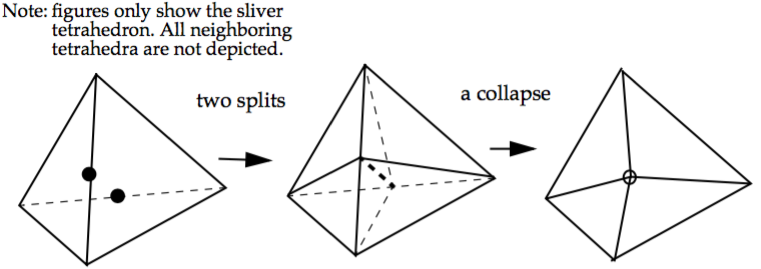
\includegraphics[width=0.8\textwidth]{split_collapse.png}
\caption{Double-split + collapse compound operator
\cite{li2003mesh}}
\label{fig:compound}
\end{center}
\end{figure}

\subsubsection{Edge Swap}
\label{sec:swap}

\begin{figure}
\begin{center}
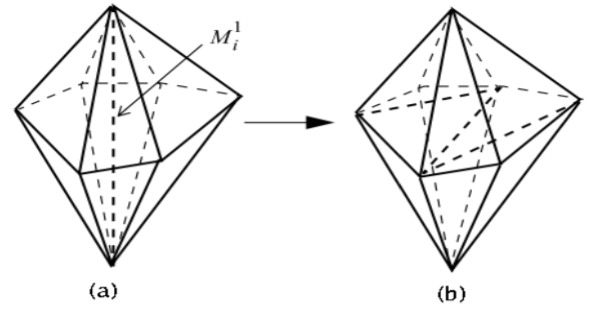
\includegraphics[width=0.5\textwidth]{swap.png}
\caption{Edge swap in tetrahedral mesh
\cite{lu2011developments}}
\label{fig:swap}
\end{center}
\end{figure}

The edge swap operation deserves a detailed consideration due
to its complexity.
Its goal is to remove the elements adjacent to an edge and
replace them with a new set of elements such that the edge
is not recreated.
In the tetrahedral case, this essentially reduces to the problem
of forming an output triangular mesh based on the ``ring" vertices
(those vertices which are opposite to the central edge across
an input triangle), as Figure \ref{fig:swap} illustrates.
Furthermore, since this operation is used almost exclusively
for the purpose of repairing quality degradation (sliver removal),
what we are interested in is finding the triangular mesh of the
ring such that the resulting tetrahedral mesh of the cavity
contains elements above a certain quality.
The quality to beat is usually the lowest quality input
tetrahedron, i.e. we want to at least improve the minimum quality.

A naive search of the space of possible triangular meshes
can be quite expensive, so we use an optimized algorithm
described by Freitag and Ollivier-Gooch \cite{freitag1997tetrahedral}.
The algorithm consists of limiting oneself to rings of a
certain number of vertices (in our case, not attempting
rings that have more than 7 vertices), and storing integer
tables describing all possible trianglulations of such rings.
The triangulations are described in terms of unique triangles
(two triangulations may share the same triangle).
Because the qualities of the two adjacent tetrahedra adjacent
to such a triangle are uniquely defined, then if either quality
is below the target threshold, all triangulations that include
that triangle can be ignored.
Otherwise, the lower of the two qualities is stored in association
with the unique triangle, to avoid later re-computation.

\subsection{Overall Steps}

Listing \ref{lst:ma} shows an abbreviated version of the C++
code for MeshAdapt's main function.
The central loop executes a fixed number of iterations.
At each iteration, we first coarsen as described
in Section \ref{sec:ma_coarsen}, followed by refinement
as described in Section \ref{sec:ma_refine}.
We perform coarsening before refinement because this
should reduce the peak memory usage between the two
operations.
Shape correction is performed after the main loop
has completed, using the algorithm in Section \ref{sec:ma_shape}.
The functions whose names end in \texttt{Balance} execute
parallel load balancing.
We treat mesh elements as the units being balanced,
and assign weights to them based on the metric space
volume defined by Equation \ref{eq:metric_volume}.
Either graph partitioners \cite{devine2002zoltan} or
diffusive partitioning methods \cite{SmithParma2015}
may be used at each step.

\begin{lstlisting}[float,style=dan-style,caption=MeshAdapt main function,label=lst:ma]
void adapt(Input* in) {
  Adapt* a = new Adapt(in);
  preBalance(a);
  for (int i = 0; i < in->maximumIterations; ++i) {
    coarsen(a);
    midBalance(a);
    refine(a);
  }
  fixElementShapes(a);
  postBalance(a);
  delete a;
  delete in;
}
\end{lstlisting}

\section{Omega\_h Methods}
\label{sec:omega_h-adapt}

The Omega\_h code aims to provide MeshAdapt-like functionality
on a wide variety of computing hardware.
Due to the restrictions introduced by parallelism, Omega\_h
initially chose a simpler set of algorithms to reduce the
cost of redesigning each algorithm for portability.

There are several key characteristics of MeshAdapt's design
which need to be changed in order to execute efficiently with
high degrees of shared memory parallelism (e.g. on GPUs):
\begin{enumerate}
\item The assumption of a persistent thread which can maintain
substantial amounts of local data (e.g. a data structure
representing a mesh partition) and act on that data in serial
is invalid for GPUs, because the increased degree of parallelism
requires lowering the per-thread overhead in memory use and computation.
Shared memory parallelism is better expressed at the loop level
(see Section \ref{sec:openmp}), and per-thread data should be avoided.
This means data storage concerns (data structures) move up to
the process level (in terms of software) and up to the
node level (in terms of hardware).
\item Modification of the mesh cannot be based on a local \emph{series}
of single entity additions and removals that are immediately
applied to the mesh, because this
introduces increasing contention on the mesh data structure
as the number of threads increase.
Most other research in shared-memory parallelization of mesh modification
has focused either on methods which assume the degree of parallelism
is somewhat small \cite{remacle2015two} (as it is in CPUs) or
methods which use entity-level non-deterministic mutual exclusion
mechanisms \cite{navarro2011parallel}.
We instead propose a deterministic independent set selection system
in Section \ref{sec:indset} that allows us to go from one
simple static structure to another
(the data structure is described in Section \ref{sec:osh_static}).
\item The operations that are performed in parallel should
avoid making use of dynamic local memory allocation
(see Section \ref{sec:cuda}).
For example, when threads need access to variable-length adjacency
data such as upward adjacencies, it is better for them to
cooperate and form a single data structure representing said
information for all entities, instead of having each thread
recompute its portion on demand during a higher-level operation.
\end{enumerate}
Altogether, this results in the need to write the entire program
in an array-based and loop-based style and requires algorithms that
are intuitively expressed in that style.

We have designed such alternative algorithms for performing mesh
adaptation, and so far they have demonstrated
equivalent and in some cases higher quality results
for simplex mesh adaptation.
Additional efforts are still underway to examine algorithmic details,
and additional test cases are being developed in collaboration with
other research groups to better qualify mesh adaptation methods
independent of parallelization.

The following sections describe the algorithms implemented
in Omega\_h in contrast to those of MeshAdapt.

\subsection{Refinement}
\label{sec:osh_refine}

Instead of using template-based refinement, Omega\_h
uses single edge splits, meaning a single edge is
bisected and adjacent elements are bisected
at a single operation.
Unlike the simultaneous execution that is possible
with template-based refinement, only edge
splits whose cavities do not overlap can be
applied simultaneously (see Section \ref{sec:indset}
for how such splits are selected).
Several researchers have similarly had success
using only single edge splits rather than
template-based refinement
\cite{compere2010mesh,loseille20093d,michal2012anisotropic}.
Like MeshAdapt, Omega\_h marks all edges whose
metric length exceeds some threshold (typically $\sqrt{2}$) as candidates
for edge splits.

However, Omega\_h unmarks any edges whose splitting
would produce elements of low mean ratio quality (typically less than $20\%$).
There is a trade-off here between two desired outcomes.
On the one hand, when mesh adaptation is used to control discretization
error, it is preferable to produce meshes of higher than desired resolution
as opposed to lower than desired (in many cases the latter is unacceptable).
Combined with the fact that refinement cannot technically produce
inverted elements or invalid meshes, this is a strong motivation to immediately
and unconditionally refine all edges that exceed a given threshold.
On the other hand, immediate refinement can produce elements of arbitrarily
bad quality, making it increasing difficult to apply future mesh modifications
and driving numerical conditioning of the physical simulation to unwanted extremes.
Since computers use finite precision arithmetic, there are cases in practice
where the resulting element volumes are indistinguishable from zero to the computer.
In Omega\_h, we choose to avoid immediate refinement that would violate
quality criteria under the assumption that subsequent
operations (including other refinements) will improve the situation
sufficiently that the deferred refinement will eventually be accepted.
We have also confirmed that this does occur by observing the maximum
metric edge length for all test cases to date.

\subsection{Coarsening}
\label{sec:osh_coarsen}

Like MeshAdapt, Omega\_h uses single edge collapses
for mesh coarsening.
Since all operations in Omega\_h use the quality-driven
independent set system described in Section \ref{sec:indset},
that explicitly takes care of the need for an independent
set of collapsing vertices.
Edge collapses have some confusion in what their ``key" entity is,
because in reality it is the combination of an edge and one
of its endpoint vertices that defines a collapse.
We first mark all edges whose metric length is beneath
some threshold (typically $1/\sqrt{2}$) as candidates to collapse
via either endpoint.
In addition, Omega\_h will mark all edges adjacent to either endpoint
of a short edge as additional candidates, since collapsing an endpoint
along one of these additional edges may still elongate it.
Then, for all candidate edges, collapses in the allowed directions are evaluated
using almost all of the checks described in Section \ref{sec:ma_coarsen}.

Omega\_h saves time by skipping the full edge ring and face
ring checks, replacing them with a requirement that each $d$-dimensional simplex
adjacent to the collapsing edge must be classified on the same geometry
as its $(d-1)$-dimensional side adjacent to the collapsing vertex.
In other words, Omega\_h checks for the problematic case shown in Figure
\ref{fig:surf_collapse}, but not for the case in Figure \ref{fig:circle_hole}.
As a result, Omega\_h requires that the input mesh, model or metric be
constructed such that the case in Figure \ref{fig:circle_hole} doesn't arise.
The simple way to ensure this is to mesh ``holes" in the geometry.
For Omega\_h's first target applications,
this makes sense because the interaction of both the fluid and the structure
is of interest.
Barring that solution, one can topologically break up periodic geometry
or use curvature-targeted metrics to ensure a periodic geometry is approximated
with more than three edges.

Finally, Omega\_h applies the same quality restriction to coarsening
that it applies to refinement, i.e. changes are not accepted if they produce elements
below a user-defined threshold.

We mark candidate collapses using two boolean flags per edge, one for each
endpoint.
In addition to unmarking collapses that would violate the above topological
and classification checks, we also require the output elements to be
above some quality threshold.
Once all collapses that violate the checks mentioned above are unmarked,
we move the focus of the problem from edges to vertices.
To do this, every vertex chooses the highest-quality candidate edge collapse
for which it is an endpoint, and that collapse is the one it will
represent, all others for which it is an endpoint are discarded.
Now the independent set selection in Section \ref{sec:indset} is used
with vertices as the keys and their selected collapse's qualities as the
values.
The selected independent set of vertices is then collapsed, along each
vertex's chosen edge.

\subsection{Shape Correction}
\label{sec:osh_shape}

Omega\_h uses simpler and yet possibly more effective shape correction logic.
We have found that it is beneficial to consider a wider portion of the
mesh surrounding a sliver when attempting to remove said sliver, rather
than being overly concerned with the particular shape of said sliver.
Omega\_h has a user-defined parameter for how many layers of elements
around a sliver will be considered.
In this case, layers are defined by elements adjacent to one another
across faces, simply because this graph is much cheaper to compute
than that of elements adjacent via vertices.
For every sliver, elements that are at most the specified distance
via face adjacency are marked as being involved in sliver removal.
Then we do one of two things:
\begin{enumerate}
\item Mark all edges of all considered elements as candidates for edge swaps.
For each such edge we compute the best possible edge swap operation
using the optimizations described in Section \ref{sec:swap},
and give those quality values to the method in Section \ref{sec:indset} to
select a set of edge swaps to perform.
Only edge swaps which locally improve the quality in their cavity are accepted.
\item Mark all vertices of all considered elements as candidates for collapsing.
For each of these vertices, we consider collapsing it along any adjacent edge.
This is just a marking process, after which the procedure in Section \ref{sec:osh_coarsen}
is carried out, with the only difference being that for a collapse to be accepted,
the quality in the cavity must locally improve, instead of being above a
constant threshold.
\end{enumerate}
Note that although these algorithms describe using layers around a sliver,
they remain cheap because the layers need only be marked, after which only
small cavities around the marked elements are considered.
The full set of elements marked around a sliver is never collected or examined
as a whole in any way.
The marking itself can be done in a local iterative fashion, each step adding
marks to all face-adjacent elements of currently marked elements.

Unlike MeshAdapt, Omega\_h requires that all elements be above a certain
mean ratio quality, and will continue to attempt shape correction until
this goal is satisfied.
So far, we have been able to achieve minimum mean ratios between $20\%$
and $30\%$ for all mesh elements in a variety of cases.

\subsection{Overall Steps}
\label{sec:osh}

Listing \ref{lst:osh} shows an abbreviated version of the C++ code for
Omega\_h's main function.
The ordering of these operations was selected for the most part to minimize
the amount of work done, not to optimize memory usage or metric conformity.
First, refinement as described in Section \ref{sec:osh_refine} is done
until no more modifications are accepted.
Next, the same is done for coarsening as per \ref{sec:osh_coarsen}.
Finally, while the lowest element quality in the mesh is below some
threshold, we attempt to apply edge swaps and edge collapses as
per \ref{sec:osh_shape}.
Notice that edge swaps are strongly preferred, in fact edge
collapses as a quality repair solution are only attempted when
quality remains below the threshold and no legal edge swaps
would improve quality.

The parameter \texttt{qual\_floor} represents the quality that
we would prefer elements to always exceed during all parts of
adaptation.
There is an exception for the case when the input mesh is
already worse than that, hence the logic for computing
\texttt{allow\_qual}, which is the quality actually enforced
on modification operations.
The parameter \texttt{qual\_ceil} is the quality we would prefer
elements exceed \emph{after} mesh adaptation, and hence is the
target for shape correction operations.

\begin{lstlisting}[float,style=dan-style,caption=Omega\_h main function,label=lst:osh]
bool adapt(Mesh* mesh, Real qual_floor, Real qual_ceil, Real len_floor,
    Real len_ceil, Int nlayers) {
  auto input_qual = mesh->min_quality();
  auto allow_qual = min2(qual_floor, input_qual);
  while (refine_by_size(mesh, len_ceil, allow_qual));
  while (coarsen_by_size(mesh, len_floor, allow_qual));
  while (mesh->min_quality() < qual_ceil) {
    if (swap_edges(mesh, qual_ceil, nlayers)) continue;
    if (coarsen_slivers(mesh, qual_ceil, nlayers)) continue;
    break;
  }
  return true;
}
\end{lstlisting}

\section{Size Field Algorithms}
\label{sec:sf}

\subsection{Metric Interpolation and Storage}
\label{sec:metric_interp}

The metric tensor field introduced in Section \ref{sec:def_metric}
is typically provided as a set of values defined at mesh vertices.
This leads to an important question about how to compute metric
tensor values at other points in the mesh, i.e. how to interpolate
the metric tensor.
We can illustrate the issues involved with the simplest interpolation
case, that of deriving a metric tensor for the center of a mesh
edge given the two metric tensors at its endpoints.
Unfortunately, linear interpolation of the components of the
tensor $\mathcal{M}$ itself has the undesirable property that
interpolating between two highly anisotropic metrics of even
slightly different orientations will tend to produce isotropic
results with very small desired lengths, i.e. the longer desired
length will be lost.
For this reason, alternative interpolation methods have been developed
focusing on getting desired results in the case of high anisotropy.
Some of the most relevant are as follows:

\begin{enumerate}
\item MeshAdapt works with an internal representation consisting
of the orthogonal matrix $R$ and the vector of desired lengths
$\mathbf{h} = (h_1, h_2, h_3)^T$ which form the metric tensor:
\begin{equation}
\mathcal{M} = R^T \begin{bmatrix}
1 / h_1^2 & 0 & 0 \\
0 & 1 / h_2^2 & 0 \\
0 & 0 & 1 / h_3^2 \\
\end{bmatrix} R
\end{equation}
Each of these is then interpolated separately.
The vector $\mathbf{h}$ is linearly interpolated, while the
matrix $R$ is first linearly interpolated, and then re-orthogonalized
using the Gram-Schmidt process \cite{trefethen1997numerical}.
The benefit of this is that anisotropy is fully preserved due to the
separate interpolation of lengths.
However, there are three main drawbacks to this method:
\begin{enumerate}
\item The interpolation of $R$ is fragile, because if the linearly
interpolated value is rank-deficient then re-orthogonalization
will fail. This can happen, for example, if the two input $R$ matrices
represent rotations that are $180^{\circ}$ away from each other.
Even though these represent exactly the same metric tensor, interpolation
would fail.
\item The overall method gives results which depend too much on the
details of how the tensor was decomposed.
If we have two metrics which are $90^{\circ}$ away from each other
as shown in Figure \ref{fig:90deg_interp},
their interpolated result depends heavily on the signs of the eigenvectors
chosen for $R$.
\item This method stores 12 components per vertex on a 3D mesh, whereas
the alternatives below store only 6.
\end{enumerate}
\item Omega\_h computes the inverse of the metric tensors, then
interpolates those linearly, and inverts the result.
This is a method proposed by Alauzet and Frey as a compromise between
the anisotropic fidelity and high runtime costs of the following two methods
\cite{alauzet2003estimateur}.
\item The highest fidelity interpolation suggested by Alauzet and Frey is
the Power method which linearly interpolate $\mathcal{M}^{-1/2}$,
which equals $\mathcal{M}$ replacing each eigenvalue $\lambda$
with $(1/\sqrt{\lambda})$.
This requires the additional expense of computing an eigendecomposition.
\item An even better fidelity interpolation suggested by Loseille and
L{\"o}hner \cite{loseille20093d} and later confirmed by
Michal and Krakos \cite{michal2012anisotropic} is the Log-Euclidean
method which linearly interpolates $\log(\mathcal{M})$, which equals
$\mathcal{M}$ replacing the eigenvalues $\lambda$ with $\log(\lambda)$.
Figure \ref{fig:log_interp} shows how this method better preserves
very high levels of anisotropy.
\end{enumerate}

\begin{figure}
\begin{center}
\includegraphics[width=0.6\textwidth]{90deg_interp.png}
\caption{MeshAdapt interpolation depends on eigenvector signs}
\label{fig:90deg_interp}
\end{center}
\end{figure}

\begin{figure}
\begin{center}
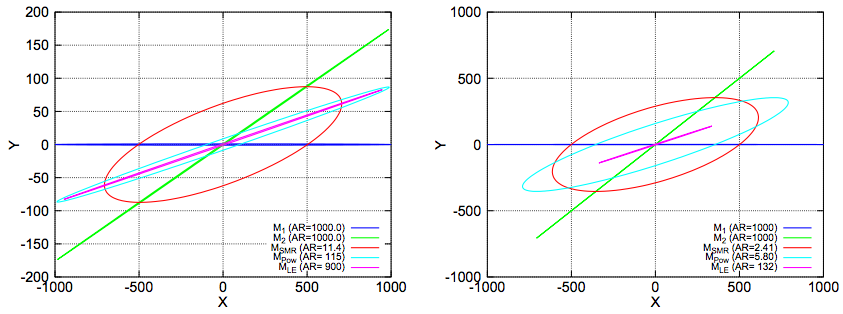
\includegraphics[width=0.95\textwidth]{log_interp.png}
\caption{Log-Euclidean versus Power interpolation
at 1:1000 anisotropy \cite{michal2012anisotropic}}
\label{fig:log_interp}
\end{center}
\end{figure}

To date the former two methods have proved sufficient for certain
degrees of anisotropy, yet we consider the implementation of one
of the latter two methods as an area of immediate future work.

\subsection{Implied Metric Field}
\label{sec:ident_metric}

It is often useful to develop an ``implied" metric field
\cite{michal2012anisotropic}.
Given a mesh, the implied metric field is the one which the mesh
currently satisfies.
Since there often does not exist a metric field which is exactly
satisfied, the computed field is an approximation of the field
which is most closely satisfied by the existing mesh.
An implied metric field can be used to maintain a mesh's
initial gradation while responding only to mesh motion.
More importantly, it can be combined with the user's desired
metric field to produce one or more intermediate metric fields
which are more suitable for mesh adaptation
(for example, gradually interpolating from one to the other).

For any simplex element, there exists a single metric tensor
such that all its edges are unit length in metric space, which
implies it is equilateral and has a perfect mean ratio quality
in metric space.
To find this metric, consider that each edge $i$ of the simplex
forms a single scalar constraint:

\begin{equation}
1 = \sqrt{\mathbf{v}_i^T \mathcal{M} \mathbf{v}_i}
\end{equation}

Where $\mathbf{v}_i$ is the real space vector along edge $i$.
Also note that the metric tensor $\mathcal{M}$ has exactly as
many independent scalars as the simplex has edges
($3$ in 2D, $6$ in 3D).
The constraint can be converted into a scalar equation
for the independent variables:

\begin{gather*}
1^2 = \left(\sqrt{\mathbf{v}_i^T \mathcal{M} \mathbf{v}_i}\right)^2 \\
1 = \mathbf{v}_i^T \mathcal{M} \mathbf{v}_i \\
1 = \begin{bmatrix} x_i & y_i & z_i \end{bmatrix}
\begin{bmatrix}
a & d & f \\
d & b & e \\
f & e & c \\
\end{bmatrix}
\begin{bmatrix}
x_i \\
y_i \\
z_i \\
\end{bmatrix} \\
1 = ax_i^2 + by_i^2 + cz_i^2 + 2dx_iy_i + 2ey_iz_i + 2fx_iz_i
\end{gather*}

This leads to a linear system, which following our 3D example
is a $6\times 6$ system:

\begin{equation}
\begin{bmatrix}
x_1^2 & y_1^2 & z_1^2 & 2x_1y_1 & 2y_1z_1 & 2x_1z_1 \\
x_2^2 & y_2^2 & z_2^2 & 2x_2y_2 & 2y_2z_2 & 2x_2z_2 \\
x_3^2 & y_3^2 & z_3^2 & 2x_3y_3 & 2y_3z_3 & 2x_3z_3 \\
x_4^2 & y_4^2 & z_4^2 & 2x_4y_4 & 2y_4z_4 & 2x_4z_4 \\
x_5^2 & y_5^2 & z_5^2 & 2x_5y_5 & 2y_5z_5 & 2x_5z_5 \\
x_6^2 & y_6^2 & z_6^2 & 2x_6y_6 & 2y_6z_6 & 2x_6z_6 \\
\end{bmatrix}
\begin{bmatrix}
a \\ b \\ c \\ d \\ e \\ f
\end{bmatrix}
\begin{bmatrix}
1 \\ 1 \\ 1 \\ 1 \\ 1 \\ 1
\end{bmatrix}
\end{equation}

Where $y_3$ is the $y$ component of the length of edge 3,
and so on.
The matrix and right hand side are formed based on the element
and the linear system is solved via QR decomposition
\cite{trefethen1997numerical}, giving us
the implied metric tensor for an element.
This derivation can be repeated for triangles in 2D, giving
a $3\time 3$ system for the symmetric tensor components.

In order to compute metric tensors at vertices,
We need to conceptually average the implied values obtained
at adjacent elements.
First, we transform the element metric tensors into their
``linear" form, which is one of the forms described
in Section \ref{sec:metric_interp} used for metric interpolation
(for example, Omega\_h uses the matrix inverse).
Then we take at each vertex the average of these linear
tensors at adjacent elements.
Applying the inverse ``de-linearizing" transformation to the resulting tensor
retries the metric tensor at the vertex.

\subsection{Implied Isotropic Size}
\label{sec:ident_size}

If we are doing isotropic adaptation, we can follow a
similar procedure to that in Section \ref{sec:ident_metric} for metric tensors,
by identifying a desired edge length for each element and averaging
this value to vertices.
This is different from the typical approach of averaging the lengths of edges
adjacent to a vertex, because only considering edges adjacent to the vertex
can produce inaccurate results at corners of even simple meshes, where the
axis-aligned edges are considered but diagonal edges are ignored.
Unlike metric tensors, there rarely exists a single desired length which is
satisfied by all edges of an element.
The approximation we use is the root-mean-square of the element's current
edge lengths ($l_{\text{RMS}}$) defined in Equations \ref{eq:tet_mean_ratio}
and \ref{eq:tri_mean_ratio}.
This is done for consistency with our method of predicting output element counts,
described in Section \ref{sec:elem_count}.

\subsection{Targeting an Element Count}
\label{sec:elem_count}

For users developing a desired metric field, it can be useful
to have the ability to scale their desired metric field such
that the resulting adapted mesh will have a certain desired number
of elements.
This is due to the limited amount of memory on computer systems;
simulations making use of supercomputers will typically approach
the limit of memory when storing their mesh.
Therefore, it is preferable to limit resolution and execute correctly
rather than exceed the memory limit in an attempt to reach high resolution.
Together with re-partitioning onto a larger amount of hardware memory,
metric field scaling should provide better control of parallel adaptive
workflows.

Pain, Umpleby, de Oliveira, and Goddard describe one such method for
predicting the number of elements produced and accordingly adjusting
the metric field \cite{pain2001tetrahedral}.
They begin with the assumption that after mesh adaptation all elements
will have metric volume $\gamma_K$, where $\gamma_K$ is the volume of
a perfectly equilateral tetrahedron with unit edge lengths.
This leads to their volumetric prediction of the new element count
$E_\text{new}$ based on the old elements $[1,E_\text{old}]$:

\begin{equation}
E_{\text{new}} = \frac{\sum_{e=1}^{E_{\text{old}}} \tilde{V}_e}{\gamma_K}
\end{equation}

Where $\tilde{V}_e$ is the volume of element $e$ in metric space,
as we defined in Equation \ref{eq:metric_volume}.
They then seek a scalar $\beta$ such that the scaled size field
$\beta\mathcal{M}$ will produce the desired number of elements
$E_\text{des}$.
They arrive at the following:

\begin{equation}
\beta = \left(\frac{\gamma_K\theta E_{\text{des}}}
{\sum_e^{E_{\text{old}}} \sqrt{\det(\mathcal{M}_e)}V_e}\right)^{2/3}
\end{equation}

Where $\theta$ is a correction factor which they state should
be set to approximately $0.85$.
We claim this correction factor is compensating for the invalidity
of the equilateral-volume assumption.
It is impossible to mesh Euclidean space with equilateral tetrahedra,
and should likewise be difficult in metric space.
We propose using the mean ratios of input elements (in metric space)
as an indication of how far typical element volumes would deviate
from the equilateral volume (recall the interpretation of the
mean ratio from Section \ref{sec:def_quality}).
Instead of summing metric space volumes $\tilde{V}_e$, we sum
the volumes that current elements would have if they were
made equilateral while their root-mean-squared edge length was preserved.
This makes them more comparable to the idealized equilateral
elements being assumed on output:

\begin{equation}
E_{\text{new}} = \frac{\sum_{e=1}^{E_{\text{old}}}
\gamma_K \tilde{l}_{e,\text{RMS}}^3}{\gamma_K}
 = \sum_{e=1}^{E_{\text{old}}} \tilde{l}_{e,\text{RMS}}^3 \\
\end{equation}

This leads to a simpler conclusion: the number of elements that
input element $e$ will become after adaptation is approximately
$\tilde{l}_{e,\text{RMS}}^d$
(see Equations \ref{eq:tet_mean_ratio} and \ref{eq:tri_mean_ratio}
for a definition).
This can be used to compute a new metric scaling factor:

\begin{equation}
\beta = \left(\frac{E_{\text{des}}}
{\sum_e^{E_{\text{old}}} \tilde{l}_{e,\text{RMS}}^d}\right)^{2/3}
\end{equation}

And can also be used to compute element weights to estimate
future memory usage for load balancing purposes.

\section{Solution Transfer in a Cavity}

Emphasize numerical / performance advantage
over full-mesh methods.
Results can be included for each particular
method if it warrants one.

\subsection{Conserving Integral Quantities}

\section{Serial Adaptation Performance}

{\bf TODO... }

%%% Local Variables:
%%% mode: latex
%%% TeX-master: t
%%% End:



%%%%%%%%%%%%%%%%%%%%%%%%%%%%%%%%%%%%%%%%%%%%%%%%%%%%%%%%%%%%%%%%%%%
%                                                                 %
%                            CHAPTER FOUR                         %
%                                                                 %
%%%%%%%%%%%%%%%%%%%%%%%%%%%%%%%%%%%%%%%%%%%%%%%%%%%%%%%%%%%%%%%%%%%

\chapter{SCALABLE PARALLEL MESH ADAPTATION}
\label{chap:parallel}

\section{Defining Scalability}
\label{sec:scalable}

It is important to first define scalability in the context of
parallel computers.
First, we define a single scalar $N$ describing the problem size.
For mesh-based simulations, the number of mesh elements
is a good approximate measure of problem size.
Then we consider any operation which would take $O(N)$ time to execute
on a single processor such as the reference computer
in Section \ref{sec:ref_comp}, and analyze the runtime bound
of this operation when it is parallelized using $P$ cooperating processes.
When this the parallel runtime is $O(N/P)$, we say the operation
has perfect linear scaling.
Linear scaling typically only occurs when the processes do not have to coordinate,
and coordination usually adds a factor $\log(P)$ to the runtime,
meaning that the operation takes $O((N/P)\log(P))$ time in parallel.

Notice that we are considering a single operation which takes $O(N)$
time in serial.
For example, a Recursive Bisection partitioning method is a
divide-and-conquer algorithm which uses $O(\log(P))$ steps, each
taking $O(N)$ time, to assign $N$ items to $P$ partitions
for a total serial runtime which is $O(N\log(P))$
(analogous to an incomplete sorting algorithm).
If the items are already well partitioned amongst $P$ processes
and we run a parallel version of this procedure to adjust the
partitioning, each $O(N)$ step becomes $O((N/P)\log(P))$
and the whole operation can be expected to take $O((N/P)\log^2(P))$.

Next, we define parallel runtime bounds which are considered non-scalable.
The simplest example is one where an $O(N)$ serial operation becomes
an $O(N)$ parallel operation, i.e. there is asymptotically no scaling.
Although trivial, an alarming number of parallel programs in production
use exhibit this degree of scaling for key parallel operations
(for example, partitioning is done is serial prior to a parallel simulation).
Such systems rely on the fact that their non-scalable operations
consume a small percentage of runtime at low degrees of parallelism
to show some speedup in practice, but ultimately run into great difficulties
for large $P$ or large $N$.
The second example is an operation which has $O(P)$ runtime in parallel.
Once again, may systems in production use today suffer from such
trivial non-scalability.
For example, it is natural when organizing communications for each process to create
an array of size $P$ with information about what is being sent to each
other process (or worse, to actually send data to every other cooperating process).
The continued use of $O(P)$ algorithms is a significant obstacle to
increasing the degree of shared memory parallelism in leadership-class supercomputers.
The issue is made worse by the fact that until fairly recently,
MPI (see Section \ref{sec:def_mpi}) itself would either use
or encourage the use of such algorithms \cite{balaji2009mpi}.
Section \ref{sec:paraops} describes how to use modern MPI
to avoid non-scalable operations during communication.

All the above considerations have analogues for the case of shared-memory programming,
in which case one can exchange the number of parallel processes $P$ for a number
of parallel threads $T$.
In the case of shared memory only, there are fewer communication concerns because
all threads may access all data directly.
Although there are Non-Uniform Memory Access (NUMA) costs incurred if threads do
not organize their data to minimize sharing, these costs are much smaller than
the cost of network communication.

\section{Parallel Operations}
\label{sec:paraops}

In this section we introduce a set of key collective parallel operations
used to write parallel programs.
All of these are scalable operations as described in Section \ref{sec:scalable}.
As such, a good approach to designing scalable programs is to use
only these operations for parallelism.

\subsection{Map}

This is the most basic parallel operation, and is included to
place our definitions in the context of the map-reduce programming model which
has gained popularity in processing Internet data sets \cite{dean2008mapreduce}.
The simplest definition of a map operation takes in an array $\mathbf{a}=\{a_0,a_1,a_2,...a_N\}$
and a unary operator $f$ and returns an array
$\mathbf{b}=\{f(a_0), f(a_1), f(a_2),...,f(a_N)\}$.

We generalize it to the idea of running $N$ independent
operations in parallel with no need for coordination.
The shared memory implementation of a map operation is the \texttt{parallel\_for}
concept introduced in Section \ref{sec:openmp}.
The need for these operations to be independent often forces the result to exist
as one or more arrays of $N$ result values.
The distributed memory implementation is anything inside a normal MPI program.
Since MPI processes always execute in parallel, anytime all processes perform
the same operation without coordination (message passing), it can be interpreted
as an implicit map operation.
This illustrates an important distinction between MPI programming and shared
memory programming: MPI is parallel by default, while shared memory programming
environments like OpenMP and CUDA are serial by default and parallelism
must be explicitly requested per operation.

The map operation is the prime example of an operation which scales
perfectly.
Assuming the operator $f$ requires $O(1)$ time, a serial execution
requires $O(N)$ time and a parallel operation over $P$ processes
and $T$ threads takes $O(N/(PT))$ time.

\subsection{Reduce}
\label{sec:reduce}

A reduction operation takes as input an array
$\mathbf{a}=\{a_0,a_1,a_2,...,a_N\}$ of scalar values and
a binary operator $\otimes$, and returns a single scalar result.
The result is related to the array entries via a binary expression tree,
and in order to allow flexibility of implementation, any valid binary
tree may be used.
Figure \ref{fig:reduce} shows two valid binaries trees an implementation
may use to reduce an array of five entries.
The value of a leaf node in this tree is the value of a unique array entry,
and the value of the non-leaf nodes is the result of applying
the binary operator to the values of its two child nodes.
The value of the root of the tree is the overall reduction result.

The left tree in Figure \ref{fig:reduce} illustrates the typical
serial reduction process of maintaining an accumulator value and
adding each consecutive array entry to it.
The right tree in Figure \ref{fig:reduce} illustrates the most theoretically
scalable implementation, i.e. a balanced tree.
Assuming we have as many parallel processes as we have array entries,
each of the $\lceil\log(N)\rceil$ layers of the balanced tree
can be evaluated simultaneously and the
runtime to evaluate the reduction is $O(\log(N))$ for arrays of size $N$.
However, the balanced tree requires $O(N)$ memory for the intermediate
result at one layer, while the serial tree can be evaluated with
a single accumulator ($O(1)$ memory).
The memory requirement is one reason why the serial tree is chosen
in cases when no parallelism is available.

If we have fewer parallel processes than array entries, we can use a hybrid mix
of the two trees in Figure \ref{fig:reduce}, where each processor
uses a serial tree to reduce $O(N/P)$ values in $O(N/P)$ time, and
then each process' local results are reduced using a balanced tree
in $O(\log(N))$ time resulting in an $O((N/P)+\log(N))$ runtime.

The binary operators used most often in Omega\_h reductions
are the sum, minimum, and maximum of the two inputs.
Notice that the ability of implementations to choose any tree
is a problem when the operator $\otimes$ is not commutative
(the result depends on the tree structure),
as is the case with typical computer implementations of floating-point summation.
Section \ref{sec:repro_sum} will describe a technique for dealing
with this issue.

\begin{figure}
\begin{center}
\includegraphics[width=0.7\textwidth]{reduce.png}
\caption{Two possible binary trees used for reduction}
\label{fig:reduce}
\end{center}
\end{figure}

The shared memory implementation of reductions is in our case
provided by the Kokkos library's \texttt{Kokkos::parallel\_reduce}
function \cite{edwards2013kokkos}.
The distributed memory implementation (which accepts a single value
per process) is provided by MPI's \texttt{MPI\_Reduce} and \texttt{MPI\_Allreduce}
functions (the later makes the result available to all processes, which is
often desired).
Combining these gives a reduction that can be expected to
complete in $O((N/(PT))+\log(PT))$ time.

\subsection{Scan}

Scan operations are key to scalable parallel programming, especially when using
arrays for storage.
Given an input array $\mathbf{a}=\{a_0, a_1, a_2, ..., a_N\}$ and a binary operator
$\otimes$, an inclusive scan returns an array $\mathbf{b}=\{b_0, b_1, b_2, ..., b_N\}$
where each $b_i=\text{reduce}(\{a_0, a_1, a_2, ..., a_i\}, \otimes)$, i.e. the
$i$-th output value is the result of reducing the first $i$ input values.
An exclusive scan differs in that the $i$-th output value is the reduction
of the first $(i-1)$ values only (meaning the first output value must be defined separately).
A scan with $(\otimes)=(+)$ is often referred to as a prefix sum.

Intuitively, a scan operation may be implemented with help from the intermediate
values of a reduction tree.
For example, the intermediate values in the serial tree (Figure \ref{fig:reduce}(left))
are exactly the output values for scanning, meaning a scan takes $O(N)$ time in serial.
Parallel scanning is a bit more complex and requires essentially traversing a
balanced tree twice (Figure \ref{fig:reduce}(right)), which still gives
it a time complexity of $O(\log(N))$ assuming as many processors as input values.

We use the \texttt{Kokkos::parallel\_scan} function to provide the shared
memory implementation of scans, and the \texttt{MPI\_Exscan} function
to provide the distributed memory implementation, which accepts one
value per process.

The utility of exclusive scans is in generating offsets for sub-groups of items in
a global collection based on the size of each subgroup.
For example, given the number of mesh elements per part, the \texttt{MPI\_Exscan}
takes $O(\log(P))$ time to returns offsets which can be used to establish a global
numbering of mesh elements without further communication.
Likewise, given the number of edges adjacent to each mesh vertex, a
\texttt{Kokkos::parallel\_scan} takes $O((N/T)\log(T))$ to produce offsets
for all vertices that allow the construction of compressed-row
storage for the vertex-to-edge adjacency (see Section \ref{sec:adj_arr}).

\subsection{Sort}
\label{sec:sort}

Although we do not yet require a full distributed memory sorting algorithm
in our work, we do have uses for sorting at the shared memory level
(see Section \ref{sec:reorder}), so we include this as a key parallel operation.
In Omega\_h, we use a slightly unusual definition of sorting:
given an array $\mathbf{k}=\{k_0,k_1,k_2,...,k_N\}$ of keys and
a strict weak ordering $(\prec)$ \cite{roberts2009applied},
return a permutation array
$\mathbf{p}=\{i_0,i_1,i_2,...,i_N\}$ which indicates
a sorted order for $\mathbf{k}$, meaning that ($k_{i_j} \prec k_{i_{j+1}}$).
We use this definition so that the permutation array can be re-used
to sort multiple other arrays that are associated with the array of keys.
We also require that the algorithm be stable (keys which are ``equal"
in the ordering $(\prec)$ retain the same relative order) for
determinism reasons.
This is especially important when other arrays are being sorted
using the permutation array.

Implementing a parallel sorting algorithm is considerably more
challenging than implementing scans and reductions.
At the time of this writing, Kokkos does not offer a highly general
sorting capability.
Instead, Omega\_h relies on the Thrust library to provide sorting functionality
on GPUs \cite{bell2011thrust}.
There several algorithms for sorting on GPUs \cite{satish2009designing},
ranging in complexity up to $O((N/T)\log^2(N))$, which we still consider
scalable.
On manycore CPUs, we use a parallel merge sort implementation provided
by researchers at Intel \cite{robinson2014parallel}.

\subsection{Exchange}
\label{sec:exch}

We use the term exchange to refer to the distributed memory operation
in which each process has a set of messages to send, each message
having a unique destination process, and these messages are exchanged
such that each process receives all the messages addressed to it
during the operation.
The difficult part of implementing an exchange is determining, for
a given destination process, the full set of messages addressed to it.
Hoefler, Siebert, and Lumsdaine \cite{hoefler2010scalable} describe
a communication-optimal algorithm for conducting a ``sparse dynamic exchange".
They define a sparse exchange as one in which the number of messages
sent from or received by any single process is $O(\log(P))$.
This is important, because if a process tries to send $O(P)$ messages
then it is impossible to execute the exchange in a scalable way.
They define a dynamic exchange as one in which the set of messages
a process must receive is unknown to that process at first, hence
the difficulty described above.

Many codes in use today solve this problem by using a variant
of the ``personalized consensus" algorithm in \cite{hoefler2010scalable},
reproduced here as Algorithm \ref{alg:pcx}.
By relying on a table (array) of size $P$, this algorithm is
non-scalable.
A scalable solution is the ``non-blocking consensus" algorithm
in \cite{hoefler2010scalable}, seen here as Algorithm \ref{alg:nbx}.
This algorithm uses synchronous sends, meaning that when a message
is received at its destination, a confirmation is returned to the
sender.
Once a process receives confirmation that all its outgoing messages
reached their destinations, it enters the non-blocking barrier.
This barrier can execute concurrently with other message traffic,
and once all processes enter it, it will signal its completion
to all processes.
Upon detecting completion, a process can be sure that all messages
in flight have been received, thus it is safe to stop waiting for
incoming messages.
The barrier must be non-blocking because in order to make progress,
processes must be able to continue receiving incoming messages
until the time of overall completion.
Knowing the communication is sparse, this algorithm runs in $O(\log(P))$
time \cite{hoefler2010scalable}.

\begin{algorithm}
\caption{Non-Blocking Consensus \cite{hoefler2010scalable}}
\label{alg:nbx}
\SetKwInOut{Input}{input}\SetKwInOut{Output}{output}
\Input{List $S$ of destinations and data}
\Output{List $R$ of received data and sources}
done$=$false\;
barrier\_active$=$false\;
\ForEach{$i \in S$}{
  start nonblocking synchronous send to process dest($i$)\;
}
\While{not (done)}{
  msg = nonblocking probe for incoming message\;
  \If{msg exists}{
    allocate buffer, receive message, add buffer to $R$\;
  }
  \eIf{barrier\_active}{
    comp $=$ test barrier for completion\;
    \lIf{comp}{done$=$true}
  }{
    \If{all sends are finished}{
      start nonblocking barrier\;
      barrier\_active$=$true\;
    }
  }
}
\end{algorithm}

\begin{algorithm}
\caption{Personalized Consensus \cite{hoefler2010scalable}}
\label{alg:pcx}
\SetKwInOut{Input}{input}\SetKwInOut{Output}{output}
\Input{List $S$ of destinations and data}
\Output{List $R$ of received data and sources}
allocate local table with $P$ entries, initialize all entries to `0'\;
\ForEach{$i \in S$}{
  set row target($i$) in local table to `1'\;
}
$g=$ global sum of my table row\;
\ForEach{$i \in S$}{
  start nonblocking sends to dest($i$)\;
}
\For{round from $1$ to $g$}{
  msg $=$ blocking probe for incoming message\;
  allocate buffer, receive message, add buffer to $R$\;
}
\end{algorithm}

Section \ref{sec:pcu_phased} describes how PUMI's communication
library, PCU, implements Algorithm \ref{alg:nbx}.
This implementation goes beyond MPI because it is designed to
allow communication between operating system threads instead
of just processes.

As of the MPI 3.0 standard, however, it is no longer necessary to
program one's own exchange algorithm, as it can be accomplished
by combining two key MPI systems:
scalable process topology (graph communicators) \cite{hoefler2011scalable},
and neighborhood collectives \cite{hoefler2012optimization}.
This is the approach taken for distributed memory exchanges
in Omega\_h.

MPI's neighborhood collective functions perform non-dynamic
exchanges, meaning that they must be informed of the incoming
as well as outgoing messages.
This is semantically the same as performing a series of single-message
sends and receives, but comes with a few benefits.
First, MPI's understanding that the messages are all to be
sent at once enables it to perform certain optimizations.
Second, the interface specifies that the data for all
outgoing messages is to be packed in a single array
(with data going to the same destination being contiguous).
This is good for integrating MPI with shared-memory
code, because the shared-memory code may efficiently prepare
the outgoing data array and may efficiently process the incoming
data array, thus minimizing the amount of work done by MPI
(which is not guaranteed to use shared-memory parallelism to
accelerate its work).
Unfortunately, the neighborhood collective exchange functions
have the name prefix \texttt{MPI\_Neighbor\_alltoall}, where
\texttt{alltoall} is too reminiscent of the non-scalable practice
of transmitting $O(P)$ messages from one processor.

The remaining problem of determining messages to receive can
be delegated to MPI's scalable process topology description
via the function \texttt{MPI\_Dist\_graph\_create}.
First, note that the above process is a graph theoretical problem
of determining incoming graph edges to a graph node when each
graph node knows only its outgoing edges.
\texttt{MPI\_Dist\_graph\_create} allows each process to specify
any subset of the edges in the communication graph, and assumes
responsibility for informing each process of all its incoming
and outgoing edges.
This is a more general and difficult problem than the one described
above, and we restrict our use of this function to having each
process specify all its outgoing edges.
Given this restriction, we assume it executes in $O(\log(P))$ time.

Note that the exchange operation does not have a clear shared-memory equivalent
in the context of Omega\_h,
because accessing shared memory directly is preferred over sending
explicit messages amongst threads.

\section{PCU: Scalable Inter-Thread Communication}
\label{sec:pcu}

{\bf attribution to the TOMS paper.}

{\bf Everything in this section needs to constantly
compare/contrast against what is in Section \ref{sec:paraops},
reinforce that its being redone for a hybrid environment}

PCU is a library that provides a parallel programming model including
parallel control functions.
Its two major functionalities are message passing that allows parallel tasks to
coordinate and thread management that extends the MPI programming model
into a hybrid MPI/thread system.

The foundation of PCU is its point-to-point message passing routines where
non-blocking synchronous message passing primitives are defined. There are
two versions, one of which is a direct interface to MPI, and the second supports
message passing between threads \cite{ibanez2014hybrid}. The two versions
are interchangeable, and PCU can change which set of them is being used at
run-time without affecting the rest of software components.

Building on the point-to-point primitives, PCU has an extensible framework for
collective operations such as reduction, broadcast, scan, and barrier.
Any collective whose communication pattern can be encoded as some kind of tree
is supported, and the most common ones come built-in to PCU.
These collectives are directly available to users.

Using both collectives and point-to-point communication, PCU provides a flexible
user interfaces similar to MPI 3.0's \texttt{MPI\_Neighbor\_alltoallw}.
The first phase
allows tasks to construct messages to multiple neighbors
at once and then send them.
The second phase ensures that neighbors
receive all the messages they have been sent.
This ``phased" communication algorithm is
conceptually the same as Algorithm \ref{alg:nbx}.

Finally, PCU has a system for creating a pool of threads within each process and
assigning them ranks the way MPI does to processes.
Users can call this API to enter a hybrid MPI+threads mode in which all the
communication APIs (point-to-point, collective, and phased) work between
threads.
These capabilities support PUMI's overall hybrid MPI+thread operation.

\subsection{Messaging Primitives in PCU}
\label{sec:pcu_p2p}

{\bf attribution to the PCU paper.}

The main unusual design choice of PCU compared to
other hybrid programming systems is
its focus on inter-thread message passing.
Since we must rebuild some of the high-level message
passing capabilities, we identify a set of primitive
operations as described by the MPI standard \cite{walker1996mpi}
which are sufficient for our applications:

\begin{enumerate}
\item Non-blocking synchronous send
\item Non-blocking send request completion test
\item Non-blocking probe
\item Blocking receive
\end{enumerate}

These conceptual message-passing primitives are independent
of their particular implementation.
Note that because we require the send operation to be synchronous,
it will complete if and only if the message is completely received at its
destination.

All the remaining algorithms rely only on these guaranteed properties
of the message passing primitives.
To develop inter-thread message passing, we implement inter-thread
message passing passing primitives.
These are currently based on calling thread-safe MPI versions of the
same primitives, but an area of future work involves implementing
more efficient primitives.

In order to use MPI itself to pass messages between threads, we require
that the implementation correctly handle self-sends.
Then, we need to encode the source and destination thread IDs into the message
metadata such that messages can be multiplexed out of a single process
and demultiplexed at their destination process.
The encoding of thread IDs makes use of the standard \texttt{MPI\_TAG} metadata
integer, which is typically a 32-bit signed integer.
We use 10 bits of this integer to encode each of the local IDs for the
source and destination threads.
This encoding of source and destination means that threads must inspect
messages with more sophisticated checking of the tag than
\texttt{MPI\_Recv}
offers, since messages arriving at the same process may be destined
for different threads within that process.
We use \texttt{MPI\_Iprobe} to inspect the tag before using
\texttt{MPI\_Recv} to commit to being the receiver.
This combined probe and conditional receive procedure is specified
in Algorithm \ref{alg:receive}.

\begin{algorithm}
\LinesNumbered
\SetKwInOut{Input}{input}\SetKwInOut{Output}{output}
\Input{pattern $P$}
\Output{received message metadata $M$ and data $b$, or null}
let message $M \gets$ non-blocking probe\;
\If{$M$ is null (there is no message)}{
  \Return null\;
}
\If{metadata of $M$ does not match $P$}{
  \Return null\;
}
allocate buffer $b$ per metadata of $M$\;
blocking receive $M$ into $b$\;
\Return $(M,b)$\;
\caption{Non-blocking pattern-match receive}
\label{alg:receive}
\end{algorithm}

\subsection{Simple Collectives in PCU}
\label{sec:pcu_coll}

{\bf attribution to the PCU paper.}

Collective operations are a necessary staple of
distributed-memory high-performance computing.
Operations such as parallel reduction, broadcast, and other collectives
are key to coordinating threads \cite{pjevsivac2007performance}.
More details on these collective algorithms and tradeoffs in their
implementation can be found in \cite{thakur2003improving}.
Non-blocking collectives are more advanced implementations which
are typically used to overlap communication and computation.
By using them, PCU benefits from this overlap.
Furthermore, in Section \ref{sec:pcu_phased}, we present an algorithm
for which blocking collectives are insufficient, and a non-blocking
implementation is not just convenient but necessary.

Since collectives are used by nearly all applications,
we place a focus on developing built-in
multithreaded collective operations based on the
inter-thread message passing primitives.

We consider three fundamental collective operations:
broadcast, reduce, and scan.
Other operations such as exclusive scan and all-reduce
can be built from the first three.
These operations were selected as the minimal subset
of collectives needed for our unstructured mesh operations.

These three collectives share many common features:
they use $O(\log n)$ steps for $n$ threads,
and at each step each thread is either idle, sending one
message, or receiving one message.
These shared characteristics make it easier to implement
all the collectives in a general framework which abstracts
away their differences, starting with the specific communication
pattern used.
A thread only needs to know which of the three actions to perform at each
step and with which thread it is communicating, if any.
This combined information is referred to as the communication pattern.

The second abstraction we can make is that of a merge operator, which is
essentially the MPI reduction operator
(e.g. \texttt{MPI\_SUM} or \texttt{MPI\_MAX}).
The merge operator modifies the local data based on incoming data.
For example, an reduction sum adds incoming values to local values.
We do not refer to it as the reduction operator because it is used
in all cases, including broadcast.
As an interesting corner case, the merge operator for broadcast simply
assigns the incoming value as the local value.

Following good software design, the communication pattern,
merge operator, and data are each specified separately
and are orthogonal from one another.
This follows the example of interfaces such as \texttt{MPI\_Reduce}.

With these abstract components specified, we can execute a collective
operation
using the non-blocking point-to-point message passing primitives
developed in Section \ref{sec:pcu_p2p}.
Although the simplicity of collectives would allow blocking primitives
to be used, using non-blocking primitives gives us a great benefit:
we obtain a non-blocking collective operation.
Such operations have been implemented before \cite{hoefler2007implementation}
and subsequently proposed for the latest MPI standard \cite{hoefler2006non}.
Our work implements hybrid threaded versions of such collectives.

Users of this system initiate a collective operation, and can interleave
computation with communication progress queries.
Communication progress consists of checking for incoming messages in the current
step and proceeding to the next step when they are received.

Non-blocking collectives are useful from the perspective of
of hiding latency, but they prove to be indispensable to
Algorithm \ref{alg:nbx}.

\subsection{Non-blocking Consensus in PCU}
\label{sec:pcu_phased}

A common problem that arises when dealing with parallel graphs,
and similar structures, such as the adjacency relations of unstructured
meshes, has to do with transporting graph, or mesh entities, from
one thread to another
due to changes in the graph or to other operations which affect
load balance.
Such transportation is specified in a one-sided,
push-driven manner, which means that each thread knows which
entities it should send to which other threads, but does
not know what it will be receiving.

Without {\it a priori} knowledge of the extent of information to be
received, it is difficult to determine when to stop receiving
information.
A thread can perform a continuous loop which receives messages,
but we must determine when to terminate that loop.

This problem has been solved previously in a slightly less efficient
manner \cite{ovcharenko2012neighborhood}, and is an important special case
of the general termination detection problem.
PCU implements an optimal solution based on Algorithm \ref{alg:nbx}
described in Section \ref{sec:exch}.
Note that Algorithm \ref{alg:nbx} overlaps all incoming message processing
with all outgoing message wait operations, so the potential for latency
hiding is maximized.

When implementing phased message passing, we also optimize performance
by buffering small messages.
Users see an interface which allows sending small amounts of data to
any destination.
The user interface of phased communication allows us to pack
all data traveling between the same pair of threads into a single message.
This is done prior to executing Algorithm \ref{alg:nbx}, which expects
that the number of messages sent $|S|$ is equal to the number of unique
destinations and the number of messages received $|R|$ is equal to the number
of unique sources.

This relation of message counts to communication neighbors (sources and
destinations) is quite useful in the process of determining runtime bounds.
This is because, due to mesh partitioning, each thread should have a small
and constant number of neighbors,
about 40 at most \cite{zhou2010petascale}.

We have shown previously that buffering small messages can greatly improve performance
due to the latency cost $\alpha$ and MPI's own management overhead per message,
especially for applications
with a tendency to send very small messages between the same pair of threads
\cite{ovcharenko2012neighborhood}.
In the case of multiple threads per process, buffering also reduces
the number of calls to \texttt{MPI\_Send} and \texttt{MPI\_Recv}, which reduces
contention for the MPI library between the threads in that process.
When these calls are protected by a lock, avoiding contention is important
\cite{mavriplis2002parallel}.

\section{Remote Copies and Owners}
\label{sec:remotes}

For distributed memory parallelism, we are required to separate our
data amongst multiple memory spaces.
In order to find a piece of data across an entire distributed memory
machine, one needs to pieces of information: which of the
memory spaces it is in, and where in that memory space it is.
The first value is provided by MPI and is called a ``rank", which is
a 32-bit integer identifying an MPI process.
In object-oriented codes, the second value is a pointer
to an object, which is a memory address (typically 64 bits).
If data is stored mainly in arrays as we do in our work,
the second value can be an integer, and can be 32 bits if
that is the size chosen for array indices.

The way we partition a mesh onto a distributed memory machine is
to have each MPI process create a data structure (one of those
described in Chapter \ref{chap:struct}) and store in it a subset
of the entities in the overall mesh.
Partitioning begins with a subset of the elements that will
reside in a given partition, and then requires that this
partition also contain all entities on the boundary of those
elements.
The choice of elements is typically such that each element resides
in exactly one partition (we call this an ``element-based" partitioning),
or an element may reside in multiple partitions (the most common
example of this is a special case we call ``ghosting").
A partitioning may be represented as a map from unique entities
to a subset of partitions (MPI ranks).
Each single mapping from a unique entity to a single partition
causes a ``copy" of that entity to be included in the data structure
on that partition.

In order to maintain an understanding of the mesh as a whole,
we need to maintain some information about which copies represent
the same unique mesh entity.
When working with a partitioned mesh, it is also very useful to
designate one of the copies that represent the same unique entity
as the owner copy, making it responsible for changes involving
that unique entity.
Figure \ref{fig:remotes} shows the two ways in which we maintain
this information.
On the left, we have the PUMI implementation in which every copy
stores a set of ``remote copies", which are links to all other copies
that represent the same unique mesh entity.
This forms a complete graph of connectivity between the copies of
one unique entity.
What Omega\_h maintains most of the time is a more sparse representation
in which each entity stores a link to its owner (which may
be itself, note the self-edge in Figure \ref{fig:remotes}(right)).
In both cases (PUMI and Omega\_h), a remote link is a pair
containing an MPI rank and an entity pointer, where the
entity pointer decomposes into one or more array indices
(see Section \ref{sec:sisc_mstruct}).

\begin{figure}[t]\vspace*{4pt}
\centerline{\includegraphics[width=0.9\textwidth]{remotes.png}}
\caption{Complete and owner-based remote links for a
4-partition mesh}\vspace*{-6pt}
\label{fig:remotes}
\end{figure}

\section{Entity-Level Communication}
\label{sec:dist}

A common operation in both PUMI and Omega\_h is to send
data in a way that can be interpreted as mesh entities
communicating with one another.
A good example of this would be mesh nodes communicating
field values to one another to add up contributions from
different mesh partitions.
In a more general sense, we would like to have communications
in which data is sent to and from many small objects,
where there are more objects than threads.

In PCU, there is no explicit support for this, but it
is straightforward to achieve by sending small messages
which begin with the entity pointer of a copy (obtained from remote
copies as described in Section \ref{sec:remotes}),
followed by the data aimed at that copy.
When receiving data using PCU, a thread will loop over these
small messages (which are packed into one large message
for the entire thread) and bring up the relevant entity for each message.

In Omega\_h, we have a more explicit implementation of
this communication pattern in an object called the \texttt{Dist},
which is short for ``distributor".
The \texttt{Dist} model is that of a directed communication graph from one set of
copies (the ``sources") to another set (the ``destinations").
The two sets may be the same, for example the copies of nodes of a
mesh communicating with one another, or they may be different, for example
the copies of vertices of the input mesh communicating with
the copies of vertices of the adapted mesh.
Each source may communicate with multiple destinations, although we
assume the number of destinations per source (and the number of sources
per destination) is bound by a small constant.
Notice that both the sources and destinations are sets of copies which
are distributed throughout the whole machine.

Along each edge of this communication graph, we will transmit
a small amount of data.
These transmissions will happen all at once.
First a type of data (integer, floating-point, etc.) and a width
(a very small constant, for example 3 values) are selected.
Then the input values for each source are provided, and the
\texttt{Dist} is responsible for relaying these to
the destinations, such that each destination can readily access
the data sent to it.
Note that this is really the exchange algorithm from
Section \ref{sec:exch}, it is simply implemented at a finer-grained level.

The \texttt{Dist} system goes through several stages in order
to complete its task, as illustrated in Figure \ref{fig:exch}.
Data begins in array in the memory space of each source rank,
with one entry per source.
It is then expanded such that there is one entry per communication graph
edge whose source is in this rank.
The array is then permuted such that data whose destinations are on
the same rank is stored contiguously.
At this point, we use the MPI 3.0 exchange mechanism described in
Section \ref{sec:exch} to send out the contents of the given
array and receive incoming data into a new array, which all
the data whose destinations are on this rank, sorted by the
rank of their sources.
This received array is permuted such that data is organized
by destination object.
Finally (and optionally), the data may be reduced such that
multiple values with the same destination become a single
value (recall the common reductions in Section \ref{sec:reduce}).

\begin{figure}[t]\vspace*{4pt}
\centerline{\includegraphics[width=0.8\textwidth]{exch.png}}
\caption{The stages of a Distributor exchange algorithm}\vspace*{-6pt}
\label{fig:exch}
\end{figure}

Figure \ref{fig:exch} illustrates well the symmetry of this process,
and the ease with which it can be executed in reverse.
This symmetry is reflected in the programming interface.
Each of the five transformations requires storing some data.
The expansion and reduction steps can each be described by an array
of offsets (see the compressed row format from Section \ref{sec:adj_arr}).
The permutation steps each store a permutation array.
Finally, the message-passing step also stores arrays describing which
portions of the input and output arrays are associated with which
MPI ranks (these are also symmetric).

The generality of this interface covers a wide variety of communication
needs.
Most of the time, we use it such that each source has a single destination
(e.g. entities to their owners), or symmetrically each destination may
have a single source (owners back to entities).
In order to create a \texttt{Dist} system, users need only specify
the destination of each source on a given rank, where destinations
are specified as pairs of rank and index (see Section \ref{sec:remotes}).
We use a shared-memory parallel sort (see Section \ref{sec:sort}) to
obtain the first permutation, by sorting these destinations by their rank.
We then construct the MPI information from the sorted ranks, and transmit
the destination indices on their own.
At the destination, we apply the mapping inversion described in
Appendix \ref{sec:invert_map} to obtain the second permutation and
the offsets used for reduction (this is where the small degree assumption
comes into play).
If there are multiple destinations per source, one need only specify
the offsets from sources to the provided destination links.

Notice that all of these data manipulation steps can be performed in
a shared-memory parallel fashion.
In the case of a machine which has a CPU and a GPU, the GPU performs
all the array transformations, and data is only copied to the CPU
in the form appropriate for MPI's neighborhood exchange.
After the exchange it returns to the GPU for the second half of the
transformations.
Despite this effective use of shared memory, it is still expensive
to set up a \texttt{Dist} system.
The ones which are most likely to be reused are those that Omega\_h
builds for communicating from copies of one dimension to their owners,
and so we cache these systems the same way adjacencies are cached
in Section \ref{sec:adj_cache}.

\section{Migration}

As described in Section \ref{sec:remotes}, a partitioned mesh
involves careful duplication of mesh entities into "copies"
in different memory spaces, and establishing the needed
links between copies of the same entity.
Creation of a partitioned mesh is handled by a procedure
called ``migration" \cite{ibanez2015pumi}.
It accepts as input a partitioned mesh (the input partitioning
may be such that the entire mesh is in a single partition),
and outputs a new partitioned mesh based on an input description
of where the user would like certain mesh elements.
This process is expected to take advantage of as much parallelism
as possible, within the constraints of the input and output
partitionings (for example, if either one has the whole mesh
in one partition, portions of the migration will be inherently serial).

Following their respective styles, PUMI will modify the given
mesh by incrementally adding and removing entities and remote
copy links,
while Omega\_h will construct a new mesh structure.

The following sub-sections cover the key sub-problems involved
in mesh migration:

\subsection{Derive Lower Dimensional Partitionings}
\label{sec:migr_down}

The user specifies only the element partitioning, and
the required partitioning for lower-dimensional entities needs to
be derived from it.
This is a set union problem: each partition will request lower-dimensional
entities adjacent to the elements it has been assigned.
These requests are sent to the owners of the lower-dimensional entities
in the input mesh, who will resolve duplicate requests (from multiple
adjacent elements on the same partition) and derive the set
of unique copies to generate.

\subsection{Create and Link New Copies}
\label{sec:migr_links}

For a given dimension, the new copies need to be set up
and related via remote copy links.
As above, the owner copy of an entity in the input mesh is responsible
for setting up these links.
This is where PUMI's task is more difficult due to it maintaining
a complete set of remote links (see Figure \ref{fig:remotes}).
PUMI uses several stages of communication to first construct
new copies, send their identities back to the old owner, and then
have the old owner transmit all copy identities to all copies (all-to-all
amongst copies is required to form a complete graph).
Omega\_h can use a subset of the \texttt{Dist} setup procedure
to establish and number all new copies (sources are old owners, destinations are
new copies defined at first by rank only).
Their identities are transmitted back to the old owners, who then
select a new owner amongst the new copies and transmit that single
identity back to all new copies (note that all three of these
communications are carried out by a single \texttt{Dist}).

\subsection{Build New Topological Adjacencies}
\label{sec:migr_topo}

Permanent topological adjacencies need to be constructed
between different dimensions (see Figures \ref{fig:adjs_mds} and
\ref{fig:adjs_osh} from Chapter \ref{chap:struct}).
This brings about an interesting consideration, which is that we
usually create adjacency information in a bottom-up fashion (vertices
are created, then edges are defined from vertices, etc.), but
partition information is specified first at elements, and then
derived in a top-down fashion.
PUMI resolves this in a V-cycle fashion, meaning that it will first
derive the new partitionings for all lower dimension in a top-down
fashion and then input all these partitionings to a bottom-up algorithm
for actually building new entities and setting up remote links.
Unlike PUMI (and APF in particular), where the interface is based on the
concept of an entity being an object, Omega\_h has no concept of entity
objects, only adjacency structures and associated data.
This allows it to loosen constraints and build adjacencies in a top-down fashion.
At each dimension $d$, it first resolves the unique copies of
$(d-1)$-dimensional entities as described in Section \ref{sec:migr_down}.
This results in an accurate prediction of the new identities (indices)
for those low-dimensional entities, which can be fed back to the
the old owners of $d$-dimensional entities, immediately forming
the new adjacency structure.
This can also be done with a single \texttt{Dist}, from old
$d$-dimensional owners to new $(d-1)$-dimensional copies.
It also sets up the partitioning for dimension $(d-1)$
(also a \texttt{Dist} as described in Section \ref{sec:migr_links}).
In this way, Omega\_h can carry out a full migration as a single
top-down iteration from elements to vertices.

\subsection{Transfer Associated Data}

Associated data in this case means classification, field data,
and other data such as the marks described in Chapter \ref{chap:adapt}.
The process of transferring these during migration is relatively
straightforward.
In PUMI, all such data is appended to the small message used
to construct a new copy.
In Omega\_h, we reuse the \texttt{Dist} from Section \ref{sec:migr_links}
to transfer each data array from the old owners to the new copies.

\section{Ghosting}
\label{sec:ghost}

As mentioned in Section \ref{sec:remotes}, mesh partitioning can
in some cases copy an element onto multiple partitions.
The term ghosting typically refers to a partitioning algorithm
that begins with an element-based partitioning (all elements
exist on only one partition) and gradually copies layers of elements
from neighboring partitions.
Formally, a partition after ghosting one layer will have copies
of all mesh elements adjacent to all $b$-dimensional entities
it had copies of before ghosting, where $b$ is called the bridge dimension.
In our work we only consider vertex bridges $(b=0)$.

The interface to PUMI's element-based migration procedure is
``push-based", meaning that each partition specifies, for each
of it current elements, a single destination partition to send
that element to.
By definition, such a specification cannot express ghosting.
Although PUMI has recently acquired ghosting capability, it was
not developed as part of this thesis and treats ghost elements
in a specialized manner.

We focus here on Omega\_h's implementation, which begins with
a migration procedure capable of handling any amount of element duplication.
The input to Omega\_h migration specifies a list of element copies
in the input mesh (which may be in other partitions) which define
the element copies desired in the newly partitioned mesh.
This way, one may request all the elements currently in the
partition plus several elements in other partitions.
Since the Omega\_h migration procedure treats element duplication
the same as duplication in lower dimensions, implementing ghosting
only requires specifying the right set of elements.
We form a graph from vertices to all adjacent elements (including
those on other partitions) by having every vertex copy send its
adjacent element identifiers to the vertex owner.
The vertex owners send back the full list of adjacent elements,
allowing partitions to request all elements adjacent to its current
vertices.

The only care that needs to be taken in the migration procedure
is to preserve the owner ranks of all entities when ghosting,
because this is the only mechanism for distinguishing ghosted
elements in case one needs to remove them and return to
an element-based partitioning.
This also gives a critical guarantee for parallelism:
after ghosting, an owned entity will have all upward adjacent
entities available as copies in shared memory.
Any computations that need to consider entities adjacent to
a central entity can be programmed without any communication,
assuming all information is present in the data structure.
As this is only true for owned entities, one need only communicate
the result of this computation from owned entities to their other
copies.
This is an alternative to the dynamic migration system
presented in Section \ref{sec:cavity_operator}.

\section{Parallel Cavity Operations}
\label{sec:cavity_sched}

When doing operations that account for higher-dimensional entities
around a lower-dimensional entity, it is useful to have a mechanism
for altering the mesh partition such that the cavity being operated
on (defined by the elements adjacent to a lower-dimensional entity)
is copied in its entirety onto at least one partition, so that this
partition can perform the computation.
In this way, the code that operates within the cavity need not change
when going from a serial (non-parallel) code to a scalable parallel code.
Section \ref{sec:ghost} above hints at how ghosting plays this role
in Omega\_h.
The equivalent system for PUMI is described in Section \ref{sec:cavity_operator}.

When the cavity operations alter mesh topology, one additionally needs
mechanisms for scheduling the application of these modifications
such that no two threads make conflicting modifications to the mesh,
and threads are made aware of changes by other threads as needed.
The following two Sections describe how this is done in PUMI and Omega\_h.

\subsection{Dynamic Migration}
\label{sec:cavity_operator}

There is a system in APF called \texttt{CavityOp} which is responsible
for carrying out dynamic mesh migration in order to apply a set
of requested cavity operations.
These operations may modify topology (e.g. MeshAdapt operators)
or they may not (e.g. averaging element values to vertices).
This system at all times maintains an element-based partitioning,
meaning that elements are copied onto only one partition.
It begins by iterating over the mesh and performing any
cavity operations for which the cavity is entirely within the
local partition (we say the cavity is local).
If the mesh is well partitioned, this should account for the majority
of desired operations.
Afterwards, it will mark any cavities which are broken up among
multiple partitions and executes a single migration that aims
to localize as many non-local cavities as possible.
These two steps are repeated until all cavities have been operated on.

Cavities are required to be centered around a certain key entity,
such as an edge or vertex.
To use this system, users supply certain low-level functions
to be executed.
The first function accepts a central key entity and returns information
about whether or not that entity represents a cavity that still needs
to be operated on and whether the required cavity is local.
If the cavity is not local, it indicates which low-entities need their
upward adjacent entities localized.
The second function is run after the first if the cavity is local,
and applies the user-defined operation.

The dynamic migration system will try to localize a cavity onto the
partition that owns the central key entity.
Repeated migration is necessary because cavities may overlap, which creates
a possibility of conflicts in which two overlapping cavities cannot be simultaneously
localized by this heuristic, because their owners are different.
We use a ranking of partitions to choose which competing partition
has its request satisfied.
This ensures at least that progress is guaranteed to be made at every iteration,
because the highest ranked partition in a conflict will have its cavity localized.
In practice, the number of iterations required is small and not dependent
on the problem size, which makes this a scalable system.

There are a few drawbacks to the dynamic migration system, however.
First, it alters the partitioning of the mesh, often significantly.
Because it is focused on satisfying locality requests, it result in
a poor partitioning (high surface areas) or even remove all elements
from a partition.
This has required us in practice to keep at least a few thousand
elements per partition to avoid partitions being emptied by dynamic migration.
Second, if the order of application of the cavity operations matters
(as it does in the case of topological modifications), dynamic migration
makes no attempt to order them intelligently; they will be applied
in the order that key entities are encountered during mesh iteration
and partition boundaries will by definition be acted upon later than
partition interiors.
This makes the results dependent on the partitioning of the mesh
and the ordering of mesh entities within a partition.

Ghosting as described in \ref{sec:ghost} can be used instead of dynamic
migration for operations that do not modify topology and
where the order in which the cavities
are processed does not matter.
The original partition is a subset of the ghosted partition
(so will never be empty), and can always be recovered afterwards.
For operations which modify topology and therefore are order-dependent
when cavities overlap,
Sections \ref{sec:indset} and \ref{sec:indset_ghost} describe a system
which depends on neither input partitioning nor traversal order of the mesh.

\subsection{Independent Sets}
\label{sec:indset}

As mentioned in Section \ref{sec:cavity_operator}, it may be beneficial
to have some control over the ordering of cavity operations in the
case when two or more cavities overlap.
In the case of topology modifications, it is often the case that
performing a modification will change topology such that overlapping
modifications that used to be possible are no longer applicable.
In this sense, the ordering also determines which operations will
definitely be applied and which may be discarded in favor of others.

The following Sections \ref{sec:indset_select} and \ref{sec:indset_ghost}
describe the algorithm used by Omega\_h to select operations to apply.
It aims to choose an independent set of operations (i.e. their cavities
do not overlap), such that they may be applied in
any order (including simultaneously) and produce the same result.
This allows us to execute each modification using fine-grained
shared-memory parallelism.
Such an approach was suggested for GPU use by Pande et al. \cite{pandea2015gpu},
although their implementation computed the independent set on the CPU.
Recall also that independent sets are used in MeshAdapt \cite{de1999parallel}
during coarsening to prevent a chain of overlapping edge collapses
from removing too many mesh elements (see Section \ref{sec:ma_coarsen}).

Similar to the dynamic migration system from Section \ref{sec:cavity_operator},
this algorithm may be repeated several times as each iteration
discards some operations that can then be reconsidered.
For example, when refining long edges as per Section \ref{sec:osh_refine},
one iteration will split a set of long edges such that no two of them
are adjacent to the same element.
There usually remain long edges after these splits, so the algorithm
is repeated after measuring the edges of the modified mesh.
In the specific case of Omega\_h, an independent set of edge collapses
would first be tried, but the concept of iteration remains the same.

\subsubsection{Selection of a Set}
\label{sec:indset_select}

We have to solve a graph independent set problem, with a graph whose
graph nodes are possible modifications around certain key entities
and the graph edges represent an overlap between their cavities,
in our case meaning the key entities are adjacent to a common element.
We have either vertices or edges as the key entities, and either
triangles or tetrahedra for elements.
Fast algorithms can construct the graph of keys that are adjacent
to a common element, which we use as the basis for our conflict graph.
(Note that the expanded cavities used in Section \ref{sec:conserve_momentum}
require more expensive algorithms to establish the conflict graph).

At the beginning of each pass, each key entity is annotated as either
being a candidate or not based on the conditions described throughout
Section \ref{sec:omega_h-adapt}.
If it is a candidate, it is annotated with its output cavity quality
(the minimum quality of any element that would be created by the modification).
We would like to resolve conflicts in a way that prefers ``better" mesh
modifications, which in this case is defined by output quality.

In 1986, Luby presented a highly parallelizable algorithm
for finding maximal independent sets of graphs \cite{luby1986simple}.
A maxim\emph{al} independent set is simply one that cannot be improved by
adding more graph nodes to it, as opposed to a maxim\emph{um} independent
set which is NP-hard to find and has the most graph nodes of any
possible independent set.
We develop a variant of Luby's algorithm that is still iterative,
where at each iteration graph nodes which are local maxima of some function
are added to the independent set.
Each vertex can, in parallel, determine whether its function value is
less than that of its neighbors, and alter its own state
(whether or not it is in the set)
with confidence that no neighbor will make an inconsistent decision.
Luby's original algorithm assigned random integers to each graph node
at each iteration.

Instead of local maxima of random numbers, we use local maxima of
output quality.
Our modified Luby iteration is listed in full detail
as Algorithm \ref{alg:indset}.
Its parallel \texttt{for} loop will have its iterations scheduled by the
current runtime (CUDA, OpenMP, etc.) onto the available hardware threads.
In the extreme case, there may be enough threads for all iterations
to execute simultaneously.
Recall that the principles of shared memory programming described
in Section \ref{sec:openmp} suggest careful control over array accesses.
All arrays involved in Algorithm \ref{alg:indset} are either read-only
or write-only, and the latter (\texttt{new\_state}) has each entry written
by one thread only, by aligning its writes with the iterations
of the parallel \texttt{for} loop.

\begin{algorithm}
 \LinesNumbered
 \SetKwInOut{Input}{input}\SetKwInOut{Output}{output}
 \SetKwData{Xadj}{xadj}\SetKwData{Adj}{adj}
 \SetKwData{In}{IN}\SetKwData{Out}{NOT\_IN}\SetKwData{Unknown}{UNKNOWN}
 \SetKwData{OldState}{old\_state}\SetKwData{NewState}{new\_state}
 \SetKwData{Begin}{begin}\SetKwData{End}{end}
 \SetKwData{Quality}{quality}\SetKwData{Vqual}{v\_qual}\SetKwData{Uqual}{u\_qual}
 \SetKwData{Global}{global}
 \Input{Conflict graph $G=(V,E)$ represented by $n$, \Xadj and \Adj}
 \Input{Current vertex state in \OldState (entries are either \In, \Out, or \Unknown)}
 \Input{Quality measure for each graph vertex in \Quality}
 \Input{Unique graph node IDs in \Global}
 \Output{Updated vertex state in \NewState}
 \For(\tcp*[f]{shared memory parallel for loop}){$v \gets 0$ \KwTo $n-1$}{
   \If{\OldState$[v] \neq$\Unknown}{
     \Return\;
   }
   \Begin $\gets$ \Xadj $[v]$\;
   \End $\gets$ \Xadj $[v + 1]$\;
   \tcp{vertices adjacent to chosen ones are rejected}
   \For{$j \gets $\Begin \KwTo \End$-1$}{
     $u \gets$\Adj$[j]$\;
     \If{\OldState$[u] =$\In}{
       \NewState$[v] \gets$\Out\;
       \Return\;
     }
   }
   \tcp{check if vertex is local maximum}
   \Vqual$\gets$\Quality$[v]$\;
   \For{$j \gets $\Begin \KwTo \End$-1$}{
     $u \gets$\Adj$[j]$\;
     \tcp{neighbor was rejected, ignore its presence}
     \lIf{\OldState$[u] =$\Out}{
       continue to next $j$
     }
     \Uqual$\gets$\Quality$[u]$\;
     \tcp{neighbor has higher quality}
     \lIf{\Uqual$>$\Vqual}{
       \Return
     }
     \tcp{neighbor has equal quality, tiebreaker by global ID}
     \lIf{$($\Uqual$=$\Vqual$)$ {\bf and } $($\Global$[u]>$\Global$[v])$}{
       \Return
     }
   }
   \tcp{only local maxima reach this line}
   \NewState$[v] \gets$\In\;
 }
 \caption{One iteration of independent set selection}
 \label{alg:indset}
\end{algorithm}

\begin{figure}[t]\vspace*{4pt}
\centerline{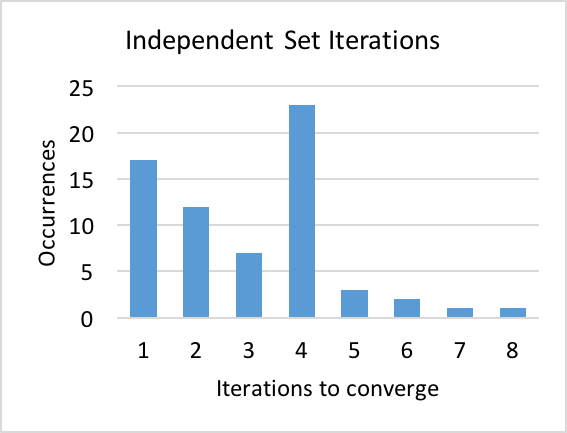
\includegraphics[width=0.5\textwidth]{indset_iters.png}}
\caption{Independent set convergence histogram}\vspace*{-6pt}
\label{fig:indset_conv}
\end{figure}

The proof of the time complexity of Luby's original algorithm
relied on probability theory and changing
the graph node numbers at each iteration \cite{luby1986simple}.
In our algorithm, the number of iterations is bounded by the
length of the longest path in the conflict graph whose nodes have monotonically
increasing quality values.
Although it may be theoretically possible to construct pathological
meshes where this path length grows proportional to the number of elements,
in practice such paths are bound by a constant.
Figure \ref{fig:indset_conv} shows a histogram of the number of
iterations required to find a maximal independent set during execution
of a typical Omega\_h mesh adaptation.
The algorithm terminates in fewer than ten iterations in all cases,
typically requiring about four iterations.

Finally, note that in line 20 of Algorithm \ref{alg:indset} we
compare graph node global IDs in the case of equal quality values.
Ties could otherwise cause the algorithm to deadlock, and we
prefer a deterministic tie-breaker.
Thus in some cases the output is affected by the global ID values,
however this does not mean it is ordering-dependent because
we update global ID values in a way that is independent
of the local ordering of entities.

\subsubsection{Ghosting for Set Selection}
\label{sec:indset_ghost}

As mentioned in Section \ref{sec:ghost}, a ghosted partition has
the useful property that every owned entity
(most importantly vertices and edges) has local copies
of all its upward adjacent entities.
All operations centered around a key entity which read information
from upward adjacent entities and write information to the
key entity can now be parallelized easily.
Every MPI rank performs the local operation around the key entities
that it owns, and then the information written to the key entities
is communicated from owned copies to all other copies.
For example, the worst element quality resulting from splitting an
edge can be evaluated locally by the MPI rank owning that edge
(because all surrounding element information is available)
and then communicated to the MPI ranks that have copies of that edge
with incomplete surrounding information.

\begin{figure}[t]\vspace*{4pt}
\centerline{
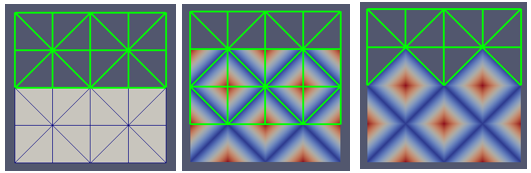
\includegraphics[width=0.7\textwidth]{mpi_indset.png}}
\caption{Steps for distributed set selection:
(left) non-ghosted partitions
(mid) add ghost layers, compute independent set
(right) trim away non-owned ghosts}\vspace*{-6pt}
\label{fig:mpi_indset}
\end{figure}

During each adaptation pass, we do what is possible without a ghost
layer first. Typically, this means measuring edge lengths and determining
whether any of them are too long or two short.
Then a ghost layer is constructed and possible operations are evaluated
as described above and an independent set is chosen as described in
Section \ref{sec:indset}.
Once an independent set has been chosen, we return to an element-based
partitioning, but one which is altered such that cavities in the independent
set reside on one MPI rank.
At that point, the code can proceed to apply the cavity modifications
and produce a new local mesh structure without further communication
because shared entities are not modified.
Figure \ref{fig:mpi_indset} illustrates this process at a simple partition boundary,
in the case of selecting which mesh vertices ought to be collapsed.

The tracking of parallel connectivity in our code is based first on global
IDs for the entities.
By the definition of our partitioning, new cavity entities are only created
inside the MPI rank which owns the cavity, so we assign their ownership
to that rank.
We can also take the intersection of entities that stayed the same
(not in cavities) and are owned.
Together these numbers give a count of how many entities in the new mesh are owned
by the local MPI rank.
A simple \texttt{MPI\_Exscan} function call converts local counts into
global numbers for owned copies.
There are still non-owned copies which do not know their global ID, but they
are by definition entities which stayed the same, so we can use the
communication instruments of the old mesh to synchronize their IDs.

Combined with the independent set selection mechanism, this results
in a mesh adaptation method which is unaffected by partition boundaries,
in the sense that the decision process of what modifications to apply
is not influenced by the partition.
The resulting algorithm is also deterministic,
in that its output is the same regardless of the order of
execution of shared memory threads and MPI processes.
Its output is independent
of ordering so long as global IDs are independent of ordering.
Most other parallel adaptation implementations that we know of explicitly
consider interior modifications first, followed by a repartitioning that
allows consideration and modification of the near-boundary mesh
\cite{loseille2015parallel,de1999parallel}, making them
partitioning-dependent.

\section{Determinism}
\label{sec:determinism}

{\bf Discuss things done by Omega\_h to achieve
determinism on heterogeneous architectures.}

\subsection{Adjacency Inversion}

{\bf The key algorithms Ben and I came up with go here.}

\subsection{Order-Independent Sums}
\label{sec:repro_sum}

%%% Local Variables:
%%% mode: latex
%%% TeX-master: t
%%% End:


%%%%%%%%%%%%%%%%%%%%%%%%%%%%%%%%%%%%%%%%%%%%%%%%%%%%%%%%%%%%%%%%%%%
%                                                                 %
%                            CHAPTER FIVE                         %
%                                                                 %
%%%%%%%%%%%%%%%%%%%%%%%%%%%%%%%%%%%%%%%%%%%%%%%%%%%%%%%%%%%%%%%%%%%

\chapter{APPLICATION TO ADAPTIVE SIMULATIONS}

\section{Workflow Integration}

Introduce how parallel adaptivity fits into workflows.

\section{PHASTA}

Possibly more than one section; just a placeholder

\section{Albany}

\section{Proteus}

\section{Alexa}

%%%%%%%%%%%%%%%%%%%%%%%%%%%%%%%%%%%%%%%%%%%%%%%%%%%%%%%%%%%%%%%%%%%
%                                                                 %
%                            CHAPTER SIX                          %
%                                                                 %
%%%%%%%%%%%%%%%%%%%%%%%%%%%%%%%%%%%%%%%%%%%%%%%%%%%%%%%%%%%%%%%%%%%

\chapter{CONCLUSIONS AND FUTURE WORK}

\section{Conclusions}

\section{Future Work}

\subsection{Convergence of PUMI and Omega\_h}

% Section \ref{sec:two_codes} presented the rationale
% for the development of Omega\_h as a separate effort,
% which opens the question of whether it is possible
% to combine the two codes in the future.
% A combination is simply defined as a code which
% has a union of their capabilities, both theoretical
% and practical.

% If a code is to make any use of current and near-future GPUs,
% then it must be written in the more restrictive programming
% model that Omega\_h operates in.
% This applies equally well to any proposed combination of the
% two codes.
% This in turn requires a redesign of algorithms
% and structures that currently violate those restrictions,
% which includes the majority of the PUMI code.

%%%%%%%%%%%%%%%%%%%%%%%%%%%%%%%%%%%%%%%%%%%%%%%%%%%%%%%%%%%%%%%%%%% 
%                                                                 %
%                           BIBLIOGRAPHY                          %
%                                                                 %
%%%%%%%%%%%%%%%%%%%%%%%%%%%%%%%%%%%%%%%%%%%%%%%%%%%%%%%%%%%%%%%%%%% 
 
%This method produces a numbered bibliography where the numbers
%correspond to the \cite commands in the text. See the LaTeX manual.
%
% \specialhead{REFERENCES}
% \begin{singlespace}
% \begin{thebibliography}{99}
% \bibitem{thisbook} This is the first item in the Bibliography.
% Let's make it very long so it takes more than one line.
% Let's make it very long so it takes more than one line.
% Let's make it very long so it takes more than one line.
% Let's make it very long so it takes more than one line. 
% \bibitem{anotherbook} The second item in the Bibliography.
% \bibitem{yetanotherbook} Another item in the Bibliography.
% \end{thebibliography}
% \end{singlespace}

% Note that, if you wish, you can use BibTeX to create your bibliography
% from a database. See section 5.6.2 of Memo RPI.110 for information. 
%%% Local Variables: 
%%% mode: latex
%%% TeX-master: t
%%% End: 

\specialhead{REFERENCES}
\bibliographystyle{unsrt} % specify bibliography style
\begin{singlespace}
\bibliography{refs}  % Prints the bibliography here, using "refs.bib"
\end{singlespace}
 % bibliography
%%%%%%%%%%%%%%%%%%%%%%%%%%%%%%%%%%%%%%%%%%%%%%%%%%%%%%%%%%%%%%%%%%%
%                                                                 %
%                            APPENDICES                           %
%                                                                 %
%%%%%%%%%%%%%%%%%%%%%%%%%%%%%%%%%%%%%%%%%%%%%%%%%%%%%%%%%%%%%%%%%%%

\appendix    % This command is used only once!
%\addcontentsline{toc}{chapter}{APPENDICES}             %toc entry  or:
\addtocontents{toc}{\parindent0pt\vskip12pt APPENDICES} %toc entry, no page #

\chapter{Theoretical Aspects}

\section{Upward Adjacency Bounds}

If geometric aspects are not taken into account, there
is limit on the number of simplices that may share a vertex.
For example, one can mesh a disk by separating it into arbitrarily
thin slices, each of which becomes a triangle.
Therefore, our proof of upper bounds on simplices sharing a vertex
must be based on an assumed geometric restriction.
We will begin with the most straightforward restriction, that
of solid angles, and correlate it to the mean ratio quality measure
defined by Equation \ref{eq:tet_mean_ratio} from Section \ref{sec:def_quality}.

\begin{equation}
\phi = \arccos\left(\frac{\cos\theta - \cos^2\theta}{\sin^2\theta}\right)
\end{equation}

\begin{equation}
\mathbf{\Omega} = 3\phi - \pi
\end{equation}

\begin{equation} \label{eq:solid_angle_degree}
n = \left\lfloor \frac{4\pi}{\mathbf{\Omega}} \right\rfloor
\end{equation}

\begin{equation} \label{eq:surf_tri_height}
h = \frac{\sqrt{3}}{2}l = \sqrt{3}\sin\left(\frac{\theta}{2}\right)
\end{equation}

\begin{equation} \label{eq:surf_tri_inradius}
r = \frac{h}{3} = \frac{1}{\sqrt{3}}\sin\left(\frac{\theta}{2}\right)
\end{equation}

\begin{equation} \label{eq:surf_tri_circumradius}
R = 2r = \frac{2}{\sqrt{3}} \sin\left(\frac{\theta}{2}\right)
\end{equation}

\begin{equation} \label{eq:surf_tri_area}
A = \frac{\sqrt{3}}{4}l^2
\end{equation}

\begin{equation} \label{eq:tet_height}
H = \sqrt{1-R^2}
\end{equation}

\begin{equation} \label{eq:tet_volume}
V = \frac13 A H
\end{equation}

\begin{equation} \label{eq:msl}
l_{\text{MS}} = \frac16(3l^2 + 3) = \frac12(l^2 + 1)
\end{equation}

\begin{equation} \label{angle_quality}
\mathcal{Q} = \left(\frac{V^2}{\gamma^2 l_{\text{MS}}^3}\right)^{\frac13}
\end{equation}
 % appendix

\end{document}
